%% %%%%%%%%%%%%%%%%%%%%%%%%%%%%%%%%%%% %%
%% Elementos Textuais (Capítulos)      %%
%% %%%%%%%%%%%%%%%%%%%%%%%%%%%%%%%%%%% %%

% Configuração para limpar cabeçalhos e manter apenas número da página
\pagestyle{fancy}
\fancyhf{} % Limpa cabeçalho e rodapé
\fancyhead[R]{\small\thepage} % Número da página no canto superior direito
\renewcommand{\headrulewidth}{0pt} % Remove linha do cabeçalho

% Força o mesmo estilo para todas as páginas (incluindo seções e capítulos)
\fancypagestyle{plain}{\fancyhf{}\fancyhead[R]{\small\thepage}\renewcommand{\headrulewidth}{0pt}}

% Força o mesmo estilo para páginas de capítulos
\fancypagestyle{chapter}{\fancyhf{}\fancyhead[R]{\small\thepage}\renewcommand{\headrulewidth}{0pt}}

% Força o mesmo estilo para páginas de seções
\fancypagestyle{section}{\fancyhf{}\fancyhead[R]{\small\thepage}\renewcommand{\headrulewidth}{0pt}}

%% Inclua aqui os capítulos que farão parte do TCC
\chapter{Introdução}\label{cha:introducao}

Em um país de dimensões continentais, o transporte rodoviário de passageiros funciona como um elemento estratégico para a integração socioeconômica, conectando municípios e garantindo a mobilidade da população \cite{FGV2023}. Enquanto o sistema interestadual é regulamentado em nível federal pela Agência Nacional de Transportes Terrestres (ANTT), conforme estabelecido em sua lei de criação \cite{BRASIL2001}, uma vasta e heterogênea rede de transporte intermunicipal opera sob jurisdição estadual.

No estado do Piauí, esta modalidade é uma realidade consolidada, cuja organização é definida pela Lei Nº 8.562 de 2025, que dispõe sobre o Sistema de Transporte Rodoviário Intermunicipal de Passageiros do Estado do Piauí (STRIP/PI). A referida lei classifica o "serviço alternativo"\ como uma das categorias oficiais do sistema, designando a Secretaria dos Transportes (SETRANS) como o poder concedente \cite{PIAUI2025}. Este serviço, prestado por veículos de menor porte, surge para suprir as lacunas deixadas pelo sistema convencional. A existência de uma legislação específica demonstra a relevância do setor, mas também evidencia a necessidade de ferramentas de gestão que se adaptem às suas particularidades operacionais.

Diante desse cenário, este trabalho propõe o desenvolvimento de uma plataforma
baseada no modelo Software como Serviço (\textit{SaaS, Software as a Service})
para a gestão integrada de empresas de transporte rodoviário alternativo.
A escolha por este modelo se fundamenta na definição de Chong e Carraro
(2006 apud \textcite{melo2007software}) como um "software implementado
como um serviço hospedado e acessado pela Internet", o que permite que empresas
utilizem soluções baseadas em nuvem com custos operacionais reduzidos e alta
escalabilidade --- características especialmente vantajosas para o setor em foco.

Este cenário, onde um serviço regulamentado e essencial como o transporte alternativo ainda opera com uma gestão predominantemente analógica — fato constatado na pesquisa de mercado realizada para este trabalho (\autoref{apendice:resultados}) —, evidencia os desafios para a modernização do setor. A ausência de sistemas de gestão integrados e a consequente dependência de processos manuais não apenas comprometem a eficiência operacional e a qualidade dos serviços prestados, mas também criam uma barreira para a inovação e o crescimento sustentável das empresas que atuam nesse segmento.

\section{Justificativa}

O transporte rodoviário alternativo de passageiros no Brasil, embora essencial para a conectividade regional, opera de forma majoritariamente analógica e fragmentada. Uma pesquisa de mercado realizada para este estudo (\autoref{apendice:resultados}) revelou que a gestão de frotas e a venda de passagens ainda são fortemente dependentes de processos manuais, como o uso de cadernos de anotações e planilhas. Essa carência de ferramentas digitais integradas limita a eficiência e o potencial de crescimento do setor. Neste contexto, a adoção de plataformas \textit{SaaS} surge como uma solução estratégica para transformar esse cenário, otimizando recursos e reduzindo custos operacionais. Estudos de mercado mais amplos corroboram essa visão, indicando que tecnologias no setor de transportes podem elevar a eficiência logística em até 15\% \cite{setcepar2023}.

Além disso, uma plataforma \textit{SaaS} voltada para o transporte alternativo pode facilitar o acesso à inovação para pequenas e médias empresas, sem exigir altos investimentos. Esse modelo permite automação da bilhetagem, gestão integrada de rotas e melhor experiência para o passageiro. Essas soluções já demonstram impacto positivo em outros segmentos do transporte, aumentando a competitividade e garantindo serviços mais confiáveis \cite{prologapp2024}. Assim, a digitalização do setor não só fortalece as empresas, mas também melhora a mobilidade interurbana, tornando os serviços mais eficientes e acessíveis.

\section{Objetivos}

\subsection{Geral}

Desenvolver um protótipo funcional de uma plataforma SaaS para a gestão integrada do transporte rodoviário alternativo de passageiros, verificando a implementação de suas funcionalidades essenciais e avaliando a usabilidade de sua interface a partir de princípios de design.

\subsection{Específicos}

\begin{itemize}
    \item Realizar uma pesquisa de mercado para identificar as dores e os processos manuais de empresas do setor de transporte alternativo;

    \item Especificar os requisitos funcionais e não funcionais de um sistema de gestão com base nas necessidades levantadas na pesquisa;

    \item Desenvolver um protótipo funcional da plataforma ViaBus, implementando os módulos de gestão de rotas, paradas, veículos, motoristas e um fluxo para agendamento de passagens;

    \item Realizar uma verificação técnica do protótipo para analisar a aderência do software aos requisitos especificados e conduzir uma avaliação heurística para identificar possíveis melhorias de usabilidade na interface.
\end{itemize}

\section{Metodologia}

A metodologia empregada para a concepção e desenvolvimento do sistema ViaBus foi estruturada em três etapas sequenciais: levantamento de requisitos, desenvolvimento do protótipo e avaliação da solução.

A primeira etapa, de levantamento de requisitos, utilizou uma abordagem mista, partindo da observação empírica do autor sobre os desafios do setor de transporte alternativo. Tais observações foram então validadas por meio de uma pesquisa de mercado qualitativa. Para tal, foi elaborado um questionário online (detalhado no \autoref{apendice:questionario}) e aplicado junto a gestores de duas empresas do setor. As respostas, consolidadas na tabela do \autoref{apendice:resultados}, foram essenciais para a especificação formal dos requisitos que nortearam o desenvolvimento.

A segunda etapa, de desenvolvimento do protótipo, seguiu um processo iterativo alinhado a práticas de prototipagem evolutiva, onde o software é construído e refinado em ciclos contínuos \cite{sommerville2011software}. Adotou-se a estratégia \textit{Frontend-First}, que prioriza a construção da interface do usuário (UI) como guia para o desenvolvimento do sistema. Utilizando o framework Next.js e a biblioteca de componentes shadcn/ui, todas as telas da aplicação foram inicialmente desenvolvidas com dados estáticos (\textit{mockados}), permitindo a validação dos fluxos de interação antes da implementação da lógica de negócio no backend.

Por fim, a terceira etapa consistiu na avaliação do protótipo. Devido à impossibilidade de realizar testes com usuários finais, optou-se por uma verificação interna em duas frentes. A primeira foi uma \textit{Verificação de Requisitos}, na qual se analisou sistematicamente o atendimento aos requisitos funcionais e não funcionais. A segunda foi uma \textit{Avaliação Heurística}, um método de inspeção consolidado para encontrar problemas de usabilidade em interfaces \cite{Nielsen1994}. Atuando como avaliador especialista, o autor inspecionou o sistema com base nas 10 heurísticas de usabilidade de Nielsen, cujos resultados detalhados são apresentados no Capítulo 5.
% % ----------------------------------------------------------
% % Fundamentação Teórica
% % ----------------------------------------------------------
% \chapter{Fundamentação Teórica}
% \label{cha:fundamentacao_teorica}

% Neste capítulo, são apresentados os conceitos essenciais que fundamentam o desenvolvimento deste trabalho. A primeira seção aborda o modelo \textit{Software as a Service} (SaaS), detalhando sua definição, arquitetura, vantagens e desafios. A segunda seção explora a aplicação de tecnologias no setor de transporte rodoviário, destacando como as plataformas SaaS podem otimizar a gestão e a eficiência operacional.

% \section{Software as a Service (SaaS)}

% O modelo \textit{Software as a Service} (SaaS), ou Software como Serviço, representa uma mudança de paradigma na forma como o software é distribuído e consumido. Em vez de adquirir licenças de uso perpétuo e instalar o software em servidores locais, os usuários acessam a aplicação pela internet, geralmente por meio de um navegador web, pagando uma taxa recorrente (assinatura) pelo serviço \cite{salesforce2025saas}.

% Nesse modelo, toda a infraestrutura subjacente — servidores, armazenamento, redes e o próprio software — é gerenciada pelo provedor do serviço. Isso significa que o fornecedor é responsável pela manutenção, atualizações, segurança e disponibilidade da aplicação, permitindo que as empresas clientes foquem em suas atividades principais sem se preocupar com a complexidade da gestão de TI \cite{microsoft2025azure}.

% \subsection{Arquitetura e Modelo de Negócio}

% A arquitetura mais comum em soluções SaaS é a \textit{multi-tenancy} (multilocação), onde uma única instância da aplicação e da infraestrutura serve a múltiplos clientes (locatários ou \textit{tenants}). Embora compartilhem os mesmos recursos computacionais, os dados de cada cliente são mantidos isolados e seguros, garantindo a privacidade e a confidencialidade das informações \cite{microsoft2025learn}. Essa abordagem permite que o provedor otimize os recursos e reduza os custos, o que se reflete em preços mais acessíveis para o cliente final.

% O modelo de negócio é baseado em assinaturas, que podem variar em preço conforme o número de usuários, os recursos contratados ou o volume de uso. Essa flexibilidade oferece escalabilidade, permitindo que as empresas ajustem o serviço de acordo com seu crescimento e suas necessidades, pagando apenas pelo que utilizam \cite{prologapp2024}.

% \subsection{Vantagens e Desafios}

% A adoção de plataformas SaaS oferece um conjunto significativo de vantagens para as empresas, especialmente para as de pequeno e médio porte, que podem não dispor de grandes orçamentos para investimentos em tecnologia. Entre os principais benefícios, destacam-se:

% \begin{itemize}
%     \item \textbf{Redução de Custos:} Elimina a necessidade de altos investimentos iniciais em hardware e licenças de software. Os custos de manutenção, atualização e suporte técnico também são responsabilidade do provedor \cite{prologapp2024}.
%     \item \textbf{Acessibilidade e Mobilidade:} Por ser acessado via internet, o software pode ser utilizado de qualquer lugar e em diferentes dispositivos, bastando uma conexão ativa.
%     \item \textbf{Escalabilidade:} As empresas podem facilmente aumentar ou diminuir a quantidade de recursos e usuários conforme a demanda, sem a necessidade de reestruturar a infraestrutura de TI.
%     \item \textbf{Atualizações Automáticas:} O provedor é responsável por manter o software atualizado com as últimas funcionalidades e correções de segurança, garantindo que todos os clientes utilizem sempre a versão mais recente da aplicação \cite{gestran2025saas}.
%     \item \textbf{Implementação Rápida:} A configuração e o início do uso de um sistema SaaS são geralmente mais rápidos em comparação com a instalação de um software tradicional (on-premise).
% \end{itemize}

% Apesar das vantagens, o modelo também apresenta desafios que devem ser considerados. A principal desvantagem é a dependência de uma conexão estável com a internet para acessar o serviço. Além disso, as opções de personalização podem ser mais limitadas em comparação com soluções desenvolvidas internamente, e a segurança dos dados, embora robusta, fica sob a responsabilidade de um terceiro, o que exige uma análise cuidadosa na escolha do fornecedor \cite{agendor2025b2b}.

% \section{Tecnologia no Setor de Transporte Rodoviário}

% O setor de transporte rodoviário de passageiros, historicamente caracterizado por processos manuais e uma gestão descentralizada, tem passado por uma profunda transformação impulsionada pela tecnologia. A digitalização das operações não apenas otimiza a gestão, mas também melhora a experiência do cliente e a segurança nas estradas.

% Ferramentas como Sistemas de Gerenciamento de Transporte (TMS, \textit{Transportation Management System}), roteirizadores inteligentes e plataformas de venda online de passagens tornaram-se cruciais para a competitividade das empresas. Um TMS, por exemplo, centraliza informações sobre frotas, motoristas, rotas e finanças, permitindo um controle mais eficaz e uma tomada de decisão baseada em dados \cite{praxio2023tecnologia}.

% \subsection{O Papel das Plataformas SaaS no Transporte}

% As plataformas SaaS surgem como uma solução ideal para democratizar o acesso a essas tecnologias avançadas no setor de transporte alternativo. Ao oferecer um sistema robusto em um modelo de serviço, as barreiras de custo e complexidade técnica são drasticamente reduzidas.

% Uma plataforma SaaS voltada para o transporte rodoviário, como a proposta neste trabalho, pode integrar diversas funcionalidades essenciais em um único ambiente. Segundo a Point Sistemas (2025), a aplicação desse modelo na logística permite obter visibilidade total da operação em tempo real, incluindo o acompanhamento de veículos, a gestão de ocorrências e a otimização de rotas com base em dados como geolocalização e tempo estimado de viagem \cite{pointsistemas2025logistica}.

% A automação de tarefas, como a emissão de bilhetes, o controle de embarque e o fechamento financeiro, reduz a incidência de erros manuais e libera a equipe para se concentrar em atividades estratégicas. Além disso, a capacidade de integrar-se facilmente com outras ferramentas, como sistemas financeiros e de CRM, cria um ecossistema tecnológico coeso e eficiente, fundamental para a modernização e o crescimento sustentável do setor \cite{gestran2025saas}.


% ----------------------------------------------------------
% Fundamentação Teórica
% ----------------------------------------------------------

\chapter{Fundamentação Teórica}
\label{cha:fundamentacao_teorica}

Neste capítulo, são apresentados os conceitos essenciais que fundamentam o desenvolvimento deste trabalho. A primeira seção aborda o modelo \textit{Software as a Service} (SaaS), detalhando sua definição, arquitetura, vantagens e desafios. A segunda seção explora a aplicação de tecnologias no setor de transporte rodoviário, e a terceira aprofunda-se na arquitetura e nas tecnologias específicas escolhidas para a construção do protótipo.

\section{Software as a Service (SaaS)}

O modelo \textit{Software as a Service} (SaaS), ou Software como Serviço, representa uma mudança de paradigma na forma como o software é distribuído e consumido. Diferentemente do modelo tradicional \textit{on-premise}, onde o cliente adquire licenças e é responsável pela infraestrutura, no modelo SaaS o cliente paga uma assinatura periódica para acessar a aplicação pela internet, que é hospedada na nuvem pelo provedor do serviço \cite{moveideias2025saas}.

Nesse modelo, toda a infraestrutura subjacente — servidores, armazenamento, redes e o próprio software — é gerenciada pelo provedor. Isso significa que o fornecedor é responsável pela manutenção, atualizações, segurança e disponibilidade da aplicação, permitindo que as empresas clientes foquem em suas atividades principais sem se preocupar com a complexidade da gestão de TI \cite{moveideias2025saas}.

\subsection{Arquitetura e Modelo de Negócio}

A arquitetura mais comum em soluções SaaS é a \textit{multi-tenancy} (multilocação), onde uma única instância da aplicação e da infraestrutura serve a múltiplos clientes (locatários ou \textit{tenants}) \cite{frontegg2021multitenant}. Embora compartilhem os mesmos recursos computacionais, os dados de cada cliente são mantidos isolados e seguros, garantindo a privacidade e a confidencialidade das informações. Essa abordagem permite que o provedor otimize os recursos e reduza os custos, o que se reflete em preços mais acessíveis para o cliente final.

O modelo de negócio é baseado em assinaturas, que podem variar em preço conforme o número de usuários, os recursos contratados ou o volume de uso. Essa flexibilidade oferece escalabilidade, permitindo que as empresas ajustem o serviço de acordo com seu crescimento e suas necessidades, pagando apenas pelo que utilizam \cite{prologapp2024saas}.

\subsection{Vantagens e Desafios para PMEs}

A adoção de plataformas SaaS oferece um conjunto significativo de vantagens estratégicas para as Pequenas e Médias Empresas (PMEs). A principal delas é a drástica \textbf{redução de custos}, pois o modelo de assinatura elimina a necessidade de altos investimentos de capital (CAPEX) em licenças e hardware, transformando-os em despesas operacionais (OPEX) previsíveis \cite{praxio2021vantagens}.

Outros benefícios incluem \cite{prologapp2024saas, praxio2021vantagens}:
\begin{itemize}
    \item \textbf{Escalabilidade e Flexibilidade:} As empresas podem facilmente aumentar ou diminuir a capacidade de uso do software para responder rapidamente às mudanças do mercado.
    \item \textbf{Acessibilidade e Mobilidade:} Por ser acessado via internet, o software pode ser utilizado de qualquer lugar e em diferentes dispositivos, algo transformador para o setor de logística, permitindo que gestores monitorem operações remotamente e equipes externas capturem dados em tempo real.
    \item \textbf{Foco no \textit{Core Business}:} Ao terceirizar a gestão da infraestrutura de TI, as PMEs podem dedicar mais tempo e recursos para a otimização das operações logísticas e atendimento ao cliente.
    \item \textbf{Segurança e Disponibilidade:} Provedores de SaaS geralmente oferecem um nível de segurança e redundância de infraestrutura superior ao que uma PME poderia implementar por conta própria, garantido por Acordos de Nível de Serviço (SLAs).
\end{itemize}

Apesar das vantagens, o modelo também apresenta desafios, como a dependência de uma conexão estável com a internet e opções de personalização potencialmente mais limitadas.

\section{Tecnologia e Inovação no Transporte Rodoviário}

O setor de transporte rodoviário de passageiros, apesar de sua importância socioeconômica, apresenta um ritmo lento na adoção de tecnologias digitais \cite{sestsenat2021relatorio}. A ausência de soluções tecnológicas integradas, especialmente no segmento alternativo, resulta em ineficiências como a falta de controle sobre os processos, a incapacidade de atender a picos de demanda e altos índices de reclamação de clientes \cite{fateczl2022impactos}.

Plataformas SaaS surgem como uma solução ideal para democratizar o acesso a tecnologias avançadas neste setor. A análise de soluções comerciais existentes, como TOTVS, iTransport e Praxio, revela uma lacuna de mercado: as ferramentas ou são muito complexas e caras para PMEs, ou são focadas em nichos específicos como o fretamento corporativo, não atendendo de forma integrada as necessidades do operador de transporte alternativo \cite{totvs2025passageiros, itransport2025gestao, praxioluna2025venda}.

\section{Arquitetura Tecnológica da Solução Proposta}

A concepção de uma plataforma robusta, escalável e de fácil manutenção depende das escolhas arquitetônicas e tecnológicas. Cada componente da arquitetura foi selecionado estrategicamente para maximizar a produtividade, garantir a qualidade do software e mitigar riscos de desenvolvimento.

\subsection{Tecnologias do Backend}

O backend é o alicerce da plataforma, responsável pela lógica de negócios, persistência de dados e segurança. A \textit{stack} escolhida foi projetada para ser modular, robusta e escalável, utilizando tecnologias consolidadas no ecossistema TypeScript.

\subsubsection{NestJS e Arquitetura Modular}
O framework escolhido para o desenvolvimento do backend foi o NestJS. Trata-se de um framework Node.js progressivo, construído com e para o TypeScript, que utiliza uma arquitetura fortemente modular \cite{nestjs2025framework}. O pilar do NestJS é o conceito de Módulos, que organizam o código em blocos coesos e funcionais (e.g., um módulo para autenticação, outro para gestão de rotas). Cada módulo encapsula seus próprios \textit{controllers}, \textit{providers} (serviços) e pode importar ou exportar funcionalidades \cite{nestjs2025modules}. Essa estrutura promove uma forte separação de responsabilidades, facilita a reutilização de código e a manutenção do sistema, sendo ideal para a plataforma proposta, onde funcionalidades complexas podem ser desenvolvidas como módulos independentes \cite{devanddeliver2024architecture}.

\subsubsection{TypeORM e Mapeamento Objeto-Relacional (ORM)}
Para a camada de persistência de dados, a escolha foi o TypeORM. Um \textit{Object-Relational Mapper} (ORM) é uma técnica que cria uma ponte entre o paradigma orientado a objetos da aplicação e o paradigma relacional dos bancos de dados, permitindo que os desenvolvedores manipulem o banco de dados através de objetos e classes, abstraindo a necessidade de escrever consultas SQL manualmente \cite{logrocket2024typeorm}. O TypeORM é um ORM maduro para o ecossistema TypeScript, que utiliza intensivamente decoradores para definir Entidades (classes que mapeiam para tabelas) de forma declarativa e fortemente tipada. Isso acelera o desenvolvimento e reduz a probabilidade de erros relacionados a dados \cite{devto2024typeorm}.

\subsubsection{Autenticação com JWT e Passport.js}
A segurança da API é um requisito crítico. A estratégia de autenticação escolhida foi baseada em \textit{JSON Web Tokens} (JWT), implementada com a biblioteca Passport.js. JWT é um padrão aberto (RFC 7519) para a criação de tokens de acesso compactos e autossuficientes. Quando um cliente faz uma requisição a um recurso protegido, ele envia o JWT, e o servidor pode verificar a assinatura para autenticar o usuário sem precisar consultar um banco de dados de sessões, resultando em uma autenticação \textit{stateless} ideal para APIs RESTful \cite{soshace2024jwt}. O Passport.js atua como um \textit{middleware} de autenticação modular, e a estratégia \textit{passport-jwt} é projetada especificamente para extrair e verificar a validade desses tokens, oferecendo uma solução robusta e padronizada para proteger as rotas da API \cite{passportjs2025jwt}.

\subsection{Tecnologias do Frontend}

A interface do usuário (\textit{frontend}) é o principal ponto de contato com os gestores e passageiros. Sua arquitetura foi projetada com foco em performance e robustez, utilizando um ecossistema moderno baseado em React.

\subsubsection{Next.js, SSR e App Router}
O framework escolhido para o frontend é o Next.js. Uma de suas principais características é o suporte nativo à Renderização no Servidor (\textit{Server-Side Rendering} - SSR), na qual a página HTML é gerada no servidor a cada requisição. Isso melhora o tempo de carregamento inicial da página e a otimização para motores de busca (SEO) \cite{medium2025ssr}. Com a introdução do \textit{App Router}, o Next.js adotou por padrão o uso de \textit{React Server Components}, que permitem que a busca de dados e a renderização de componentes não interativos ocorram exclusivamente no servidor. Isso resulta em uma redução significativa da quantidade de JavaScript enviada ao cliente e otimiza a performance geral da aplicação \cite{nextjs2025servercomponents}.

\subsubsection{React, TypeScript e Ecossistema de UI}
A base da interface é o React, uma biblioteca JavaScript para a construção de interfaces baseada em um modelo de componentes reutilizáveis. Para garantir a robustez e a manutenibilidade, o React é utilizado com o TypeScript, um superconjunto do JavaScript que adiciona tipagem estática. O TypeScript permite a detecção de erros em tempo de compilação e serve como uma forma de documentação viva, tornando o código mais fácil de entender e facilitando a colaboração \cite{dhiwise2024reacttypescript}.

Para a estilização, foi adotado o Tailwind CSS, um framework \textit{utility-first} que acelera o desenvolvimento e garante consistência visual \cite{medium2025cssframeworks}. Comple-mentando-o, a biblioteca de componentes \textit{shadcn/ui} foi utilizada. Diferente de bibliotecas tradicionais, seus componentes são copiados para o código-fonte do projeto, dando ao desenvolvedor controle total sobre o código e permitindo personalizações profundas sem \textit{vendor lock-in} \cite{shadcnui2025docs}.

\subsubsection{Gerenciamento de Formulários e Validação}
Para a gestão de formulários e a validação de dados, foi utilizada a combinação do React Hook Form com a biblioteca Zod. O React Hook Form se destaca pela sua performance, minimizando re-renderizações desnecessárias \cite{reacthookform2025getstarted}. O Zod é uma biblioteca de validação de esquemas \textit{TypeScript-first} que permite definir regras de validação de forma declarativa e, a partir delas, inferir automaticamente os tipos TypeScript correspondentes. A integração entre as duas cria um sistema de validação de formulários poderoso e com segurança de tipos de ponta a ponta \cite{contentful2024zod}.

\subsection{Conteinerização com Docker}

Para garantir a consistência do ambiente de desenvolvimento e simplificar o processo de implantação, a aplicação e seus serviços dependentes (como o banco de dados) foram conteinerizados usando Docker. O Docker é uma plataforma que permite empacotar uma aplicação e todas as suas dependências em uma unidade padronizada e isolada chamada contêiner. Isso garante que a aplicação funcione da mesma forma em qualquer ambiente, seja na máquina de um desenvolvedor ou em produção, eliminando o clássico problema de "funciona na minha máquina" \cite{docker2025overview}. Através de arquivos de configuração como o \texttt{Dockerfile} (que descreve como construir a imagem da aplicação) e o \texttt{docker-compose.yml} (que orquestra múltiplos contêineres), o processo de setup e implantação é simplificado e padronizado.

\chapter{Requisitos do Sistema}

Este capítulo apresenta a especificação dos requisitos funcionais e não funcionais do sistema ViaBus, obtidos através da pesquisa de mercado realizada e da experiência prática no setor de transporte de passageiros. Os requisitos foram organizados de forma a atender aos principais desafios operacionais identificados no levantamento de necessidades junto às empresas do setor.
\section{Requisitos Funcionais}

Os requisitos funcionais descrevem as funcionalidades que o sistema ViaBus deve executar. A \autoref{tab:requisitos-funcionais} apresenta os requisitos organizados por módulos funcionais.

\begin{table}[htbp]
  \centering
  \caption{Requisitos funcionais do sistema ViaBus}
  \label{tab:requisitos-funcionais}
  \resizebox{\textwidth}{!}{%
    \begin{tabular}{|c|l|p{8cm}|}
      \hline
      \textbf{ID} & \textbf{Módulo}      & \textbf{Descrição}                                     \\
      \hline
      \multicolumn{3}{|c|}{\textbf{Autenticação e Autorização}}                                   \\
      \hline
      RF01        & Registro             & Cadastro de usuários com validação de dados            \\
      RF02        & Login                & Autenticação segura via e-mail e senha                 \\
      RF03        & Permissões           & Controle de acesso com diferentes níveis de usuário    \\
      \hline
      \multicolumn{3}{|c|}{\textbf{Gestão Multi-empresa}}                                         \\
      \hline
      RF04        & Empresas             & Criação e gestão de perfis de empresa                  \\
      RF05        & Isolamento           & Separação completa de dados entre empresas             \\
      \hline
      \multicolumn{3}{|c|}{\textbf{Gestão de Recursos}}                                           \\
      \hline
      RF06        & Motoristas           & CRUD de motoristas com dados pessoais e profissionais  \\
      RF07        & Veículos             & CRUD de veículos com informações técnicas e manutenção \\
      RF08        & Paradas              & CRUD de pontos de parada com geolocalização            \\
      \hline
      \multicolumn{3}{|c|}{\textbf{Gestão de Rotas}}                                              \\
      \hline
      RF09        & Rotas                & Criação de rotas com sequência de paradas              \\
      RF10        & Horários             & Associação de horários e preços às rotas               \\
      RF11        & Mapas                & Visualização de rotas e paradas em mapas interativos   \\
      \hline
      \multicolumn{3}{|c|}{\textbf{Gestão de Viagens}}                                            \\
      \hline
      RF12        & Agendamento          & Criação de viagens baseadas em rotas e horários        \\
      RF13        & Atribuição           & Associação de veículos e motoristas às viagens         \\
      RF14        & Status               & Controle de status das viagens em tempo real           \\
      \hline
      \multicolumn{3}{|c|}{\textbf{Venda de Passagens}}                                           \\
      \hline
      RF15        & Interface Guiada     & Wizard para venda com fluxo orientado                  \\
      RF16        & Embarque/Desembarque & Seleção flexível de pontos na rota                     \\
      RF17        & Passageiros          & Cadastro completo dos dados dos passageiros            \\
      RF18        & Anti-Overbooking     & Verificação automática de disponibilidade              \\
      \hline
      \multicolumn{3}{|c|}{\textbf{Relatórios e Consultas}}                                       \\
      \hline
      RF19        & Listas               & Geração de listas de passageiros por viagem            \\
      RF20        & Busca                & Pesquisa avançada com múltiplos filtros                \\
      RF21        & Ocupação             & Visualização em tempo real da ocupação                 \\
      \hline
    \end{tabular}
  }
\end{table}

\section{Requisitos Não Funcionais}

Os requisitos não funcionais definem os critérios de qualidade e restrições técnicas que o sistema deve atender. A \autoref{tab:requisitos-nao-funcionais} apresenta esses requisitos organizados por categorias.

\begin{table}[htbp]
  \centering
  \caption{Requisitos não funcionais do sistema ViaBus}
  \label{tab:requisitos-nao-funcionais}
  \resizebox{\textwidth}{!}{%
    \begin{tabular}{|c|l|p{9cm}|}
      \hline
      \textbf{ID} & \textbf{Categoria} & \textbf{Descrição}                                                      \\
      \hline
      \multicolumn{3}{|c|}{\textbf{Usabilidade}}                                                                 \\
      \hline
      RNF01       & Responsividade     & Interface adaptável a diferentes dispositivos e tamanhos de tela        \\
      RNF02       & Navegação          & Interface intuitiva com navegação clara e feedback visual adequado      \\
      RNF03       & Acessibilidade     & Formulários guiados com indicadores de progresso em processos complexos \\
      \hline
      \multicolumn{3}{|c|}{\textbf{Segurança}}                                                                   \\
      \hline
      RNF04       & Autenticação       & Sistema de login seguro com controle de sessões                         \\
      RNF05       & Autorização        & Controle de acesso baseado em perfis de usuário                         \\
      RNF06       & Isolamento         & Separação total de dados entre diferentes empresas                      \\
      RNF07       & Validação          & Validação rigorosa de todas as entradas de dados                        \\
      \hline
      \multicolumn{3}{|c|}{\textbf{Performance}}                                                                 \\
      \hline
      RNF08       & Carregamento       & Tempo de resposta adequado para carregamento de páginas                 \\
      RNF09       & Consultas          & Otimização de consultas ao banco de dados                               \\
      RNF10       & Escalabilidade     & Suporte a crescimento do volume de dados e usuários                     \\
      \hline
      \multicolumn{3}{|c|}{\textbf{Manutenibilidade}}                                                            \\
      \hline
      RNF11       & Arquitetura        & Código organizado em módulos bem definidos                              \\
      RNF12       & Padrões            & Seguimento de padrões de codificação estabelecidos                      \\
      RNF13       & Documentação       & API e código adequadamente documentados                                 \\
      \hline
      \multicolumn{3}{|c|}{\textbf{Portabilidade}}                                                               \\
      \hline
      RNF14       & Containerização    & Sistema deployável em containers para diferentes ambientes              \\
      RNF15       & Configuração       & Suporte a múltiplos ambientes (desenvolvimento, teste, produção)        \\
      RNF16       & Banco de Dados     & Compatibilidade com diferentes sistemas de banco de dados               \\
      \hline
    \end{tabular}
  }
\end{table}

% ----------------------------------------------------------
% Tecnologias Envolvidas
% ----------------------------------------------------------
\chapter{Tecnologias Envolvidas} \label{cha:tecnologias}

Aqui, descreva as tecnologias, linguagens de programação, frameworks, bibliotecas e ferramentas utilizadas no desenvolvimento do projeto. Explique por que cada uma foi escolhida e como elas contribuem para o sucesso do projeto. Inclua também informações sobre bancos de dados, servidores e outras tecnologias relevantes.

\section{Título da Seção SECUNDÁRIA}



Exemplo de gráfico:



\begin{figure}[H]
\renewcommand{\figurename}{Gráfico}	
\caption*{ \label{graf2}Gráfico 2 – Distribuição do número de matrículas por etapas da 
educação básica município de Avaré – 2014}
	\begin{center}
	    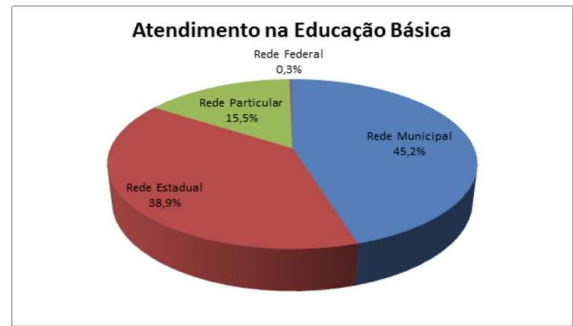
\includegraphics[scale=1.0]{imagens/grafs_1.png}
	\end{center}
	\legend{Fonte: Secretaria Municipal de Educação de Avaré (2014). }

\end{figure}

\renewcommand{\figurename}{Figura}	

\setcounter{secnumdepth}{4}

\subsection{Título da seção terciária}

Exemplo de figura:

\begin{figure}[H]
	\caption{\label{fig_arranjo}Arranjo produtivo local da banana orgânica.}
	\begin{center}
	    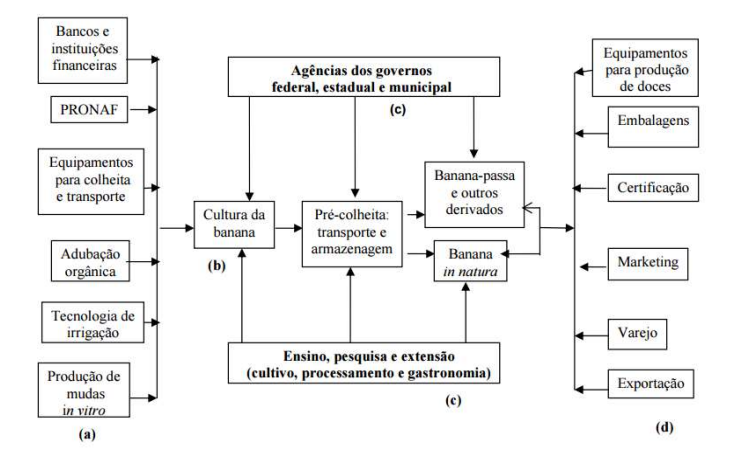
\includegraphics[scale=1.0]{imagens/fig_exemplo.png}
	\end{center}
	\legend{Fonte: \cite{limaarranjo}}
\end{figure}


% ----------------------------------------------------------
% Tecnologias Envolvidas
% ----------------------------------------------------------
\chapter{Arquitetura e Modelagem do Sistema} \label{cha:arquitetura}

\section{Arquitetura da Solução}
Esta seção descreve a organização estrutural do sistema BusLy, que provê funções de gestão de transporte para empresas: cadastro de empresas, usuários, motoristas, veículos, rotas, paradas, viagens e bilhetes. A solução adota uma arquitetura web em camadas, com separação clara entre apresentação (frontend), lógica de negócio e APIs (backend) e persistência (banco de dados).

No \textit{frontend}, utiliza-se Next.js~15 com roteamento via App Router, estado de sessão via NextAuth (estratégia \textit{JWT}) e componentes React tipados (TypeScript). O \textit{frontend} consome APIs REST autenticadas, mantém contexto de usuário/empresa e incorpora mapas e edição geográfica com Leaflet/React-Leaflet para operações sobre rotas e paradas.

O \textit{backend} é implementado com NestJS~11, estruturado por módulos de domínio (\textit{auth}, \textit{users}, \textit{companies}, \textit{drivers}, \textit{vehicles}, \textit{stops}, \textit{routes}, \textit{trips}, \textit{tickets}, etc.). As regras de negócio são expostas por controladores REST, protegidos por autenticação \textit{JWT} e autorização baseada em papéis. A multiempresa é tratada por \textit{companyId} e por um interceptor que injeta o contexto de empresa a partir do token. A persistência usa TypeORM com PostgreSQL.

\begin{figure}[H]
\centering
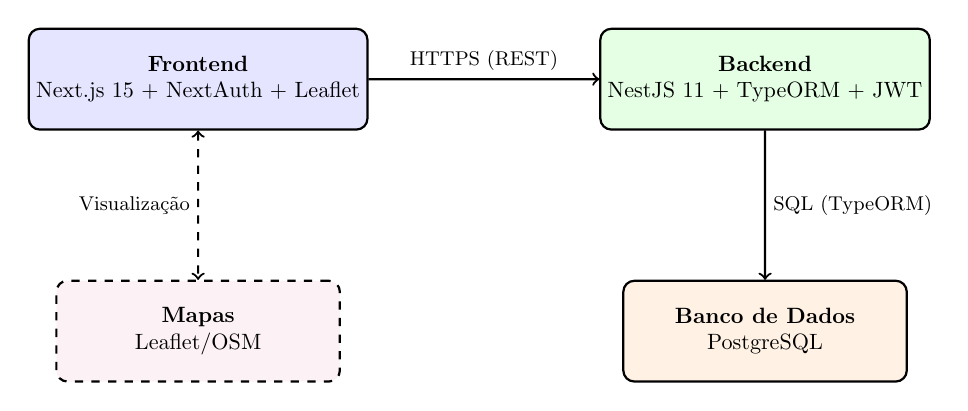
\begin{tikzpicture}[scale=0.8, every node/.style={transform shape}]
  \tikzumlset{font=\footnotesize}
  % Blocos
  \node[draw, rounded corners, thick, fill=blue!10, minimum width=4.5cm, minimum height=1.6cm, align=center] (fe) at (0,2) {\textbf{Frontend}\\Next.js 15 + NextAuth + Leaflet};
  \node[draw, rounded corners, thick, fill=green!10, minimum width=4.5cm, minimum height=1.6cm, align=center] (be) at (9,2) {\textbf{Backend}\\NestJS 11 + TypeORM + JWT};
  \node[draw, rounded corners, thick, fill=orange!10, minimum width=4.5cm, minimum height=1.6cm, align=center] (db) at (9,-2) {\textbf{Banco de Dados}\\PostgreSQL};
  \node[draw, dashed, rounded corners, thick, fill=purple!5, minimum width=4.5cm, minimum height=1.6cm, align=center] (maps) at (0,-2) {\textbf{Mapas}\\Leaflet/OSM};

  % Conexões
  \draw[->, thick] (fe) -- node[above, font=\small]{HTTPS (REST)} (be);
  \draw[->, thick] (be) -- node[right, font=\small]{SQL (TypeORM)} (db);
  \draw[<->, thick, dashed] (fe) -- node[left, font=\small]{Visualização} (maps);
\end{tikzpicture}
\caption{Visão de alto nível da solução.}
\end{figure}

\section{Modelagem do Banco de Dados}
O modelo de dados foi projetado para refletir as agregações de negócio. A Tabela~\ref{tab:principais-entidades} sumariza as principais entidades e seus papéis. De forma geral, todas as entidades operacionais são associadas a uma empresa (\textit{multi-tenancy} por chave estrangeira \texttt{company\_id}). Rotas possuem paradas ordenadas (\texttt{route\_stops}) e agenda de operação (\texttt{route\_schedules}); viagens instanciam rotas em horários específicos e originam bilhetes.

\begin{table}[H]
\centering
\begin{tabular}{ll}
\toprule
\textbf{Entidade} & \textbf{Descrição resumida} \\
\midrule
\texttt{companies} & Empresa (razão social, nome fantasia, CNPJ, slug, contato) \\
\texttt{users} & Usuário (nome, e-mail, senha, papel, status, \texttt{company\_id}) \\
\texttt{drivers} & Motorista (CPF, CNH, categoria, status, \texttt{company\_id}) \\
\texttt{vehicles} & Veículo (placa, capacidade, categoria, status, \texttt{company\_id}) \\
\texttt{addresses} & Endereço (CEP, logradouro, geocoordenadas) \\
\texttt{stops} & Parada (nome, \texttt{address\_id}, acessibilidade, \texttt{company\_id}) \\
\texttt{routes} & Rota (nome, distância, duração estimada, \texttt{company\_id}) \\
\texttt{route\_stops} & Associação rota–parada com ordem e horário opcional \\
\texttt{route\_schedules} & Agenda por dia da semana para a rota \\
\texttt{trips} & Viagem (rota, janelas horárias, status, assentos, \texttt{company\_id}) \\
\texttt{tickets} & Bilhete (passageiro, preço, assento, pontos de embarque) \\
\bottomrule
\end{tabular}
\caption{Principais entidades do domínio.}
\label{tab:principais-entidades}
\end{table}

O diagrama de classes da Figura~\ref{fig:uml-dominio} sintetiza os relacionamentos mais relevantes do domínio.

\begin{figure}[H]
\centering
\begin{tikzpicture}[scale=0.4, every node/.style={transform shape}]
  \tikzumlset{font=\tiny}
  
  % NÍVEL 1: Empresa (topo da hierarquia)
  \umlclass[x=18,y=25]{Company}{
    id: uuid\\
    legalName: string\\
    tradeName: string\\
    slug: string\\
    cnpj: string\\
    email: string\\
    phone: string\\
    logoUrl: string\\
    createdAt: Date\\
    updatedAt: Date
  }{ }
  
  % NÍVEL 2: Gestão de usuários e recursos
  \umlclass[x=3,y=18]{User}{
    id: uuid\\
    name: string\\
    email: string\\
    phone: string\\
    photoUrl: string\\
    password: string\\
    role: UserRole\\
    status: UserStatus\\
    companyId: uuid\\
    createdAt: Date\\
    updatedAt: Date
  }{ }
  
  \umlclass[x=18,y=18]{Vehicle}{
    id: uuid\\
    plate: string\\
    model: string\\
    brand: string\\
    year: number\\
    capacity: number\\
    category: VehicleCategory\\
    comfortConfiguration: ComfortConfiguration\\
    busType: BusType\\
    acquisitionDate: Date\\
    odometer: number\\
    lastMaintenance: Date\\
    nextMaintenance: Date\\
    status: VehicleStatus\\
    notes: string\\
    companyId: uuid
  }{ }
  
  \umlclass[x=33,y=18]{Driver}{
    id: uuid\\
    name: string\\
    cpf: string\\
    licenseNumber: string\\
    licenseCategory: string\\
    licenseExpiry: Date\\
    phone: string\\
    email: string\\
    birthDate: Date\\
    hireDate: Date\\
    status: DriverStatus\\
    emergencyContactName: string\\
    emergencyContactPhone: string\\
    address: string\\
    notes: string\\
    companyId: uuid
  }{ }
  
  % NÍVEL 3: Configuração de rotas
  \umlclass[x=8,y=11]{Route}{
    id: uuid\\
    name: string\\
    description: string\\
    isActive: boolean\\
    estimatedDuration: string\\
    distance: number\\
    companyId: uuid
  }{ }
  
  \umlclass[x=23,y=11]{Stop}{
    id: uuid\\
    name: string\\
    addressId: uuid\\
    isActive: boolean\\
    hasAccessibility: boolean\\
    hasShelter: boolean\\
    companyId: uuid
  }{ }
  
  \umlclass[x=38,y=11]{Address}{
    id: uuid\\
    cep: string\\
    street: string\\
    number: string\\
    complement: string\\
    neighborhood: string\\
    city: string\\
    state: string\\
    longitude: number\\
    latitude: number\\
    createdAt: Date\\
    updatedAt: Date
  }{ }
  
  % NÍVEL 4: Relacionamentos de configuração
  \umlclass[x=8,y=4]{RouteSchedule}{
    id: uuid\\
    routeId: uuid\\
    dayOfWeek: number\\
    isActive: boolean\\
    createdAt: Date\\
    updatedAt: Date
  }{ }
  
  \umlclass[x=23,y=4]{RouteStop}{
    id: uuid\\
    routeId: uuid\\
    stopId: uuid\\
    order: number\\
    departureTime: string
  }{ }
  
  % NÍVEL 5: Operação - Viagens
  \umlclass[x=3,y=-3]{TripVehicle}{
    id: uuid\\
    tripId: uuid\\
    vehicleId: uuid\\
    primaryDriverId: uuid\\
    secondaryDriverId: uuid\\
    isActive: boolean\\
    observations: string\\
    createdAt: Date\\
    updatedAt: Date
  }{ }
  
  \umlclass[x=18,y=-3]{Trip}{
    id: uuid\\
    routeId: uuid\\
    departureTime: Date\\
    estimatedArrivalTime: Date\\
    actualDepartureTime: Date\\
    actualArrivalTime: Date\\
    status: TripStatus\\
    basePrice: number\\
    totalSeats: number\\
    availableSeats: number\\
    isAutoGenerated: boolean\\
    observations: string\\
    companyId: uuid\\
    createdAt: Date\\
    updatedAt: Date
  }{ }
  
  % NÍVEL 6: Vendas - Bilhetes
  \umlclass[x=33,y=-3]{Ticket}{
    id: uuid\\
    tripId: uuid\\
    passengerName: string\\
    passengerDocument: string\\
    passengerPhone: string\\
    passengerEmail: string\\
    seatNumber: string\\
    price: number\\
    status: TicketStatus\\
    boardingPointType: BoardingPointType\\
    boardingStopId: uuid\\
    boardingLocationDescription: string\\
    boardingLatitude: number\\
    boardingLongitude: number\\
    landingPointType: BoardingPointType\\
    landingStopId: uuid\\
    landingLocationDescription: string\\
    landingLatitude: number\\
    landingLongitude: number\\
    observations: string\\
    companyId: uuid
  }{ }

  % RELACIONAMENTOS HIERÁRQUICOS PRINCIPAIS
  % Company -> Recursos
  \umlassoc[mult1=1,mult2=*]{Company}{User}
  \umlassoc[mult1=1,mult2=*]{Company}{Vehicle}
  \umlassoc[mult1=1,mult2=*]{Company}{Driver}
  
  % Company -> Configuração
  \umlassoc[mult1=1,mult2=*,arm1=-135,arm2=90]{Company}{Route}
  \umlassoc[mult1=1,mult2=*,arm1=-45,arm2=90]{Company}{Stop}
  
  % Configuração de endereços
  \umlassoc[mult1=1,mult2=*]{Address}{Stop}
  
  % FLUXO PRINCIPAL: Route -> RouteStop <- Stop
  \umlassoc[mult1=1,mult2=*]{Route}{RouteStop}
  \umlassoc[mult1=1,mult2=*]{Stop}{RouteStop}
  
  % Horários das rotas
  \umlassoc[mult1=1,mult2=*]{Route}{RouteSchedule}
  
  % FLUXO OPERACIONAL: Route -> Trip
  \umlassoc[mult1=1,mult2=*]{Route}{Trip}
  \umlassoc[mult1=1,mult2=*,arm1=-135,arm2=90]{Company}{Trip}
  
  % Trip -> TripVehicle (associação veículo/motorista)
  \umlassoc[mult1=1,mult2=*]{Trip}{TripVehicle}
  \umlassoc[mult1=1,mult2=*,arm1=-90,arm2=90]{Vehicle}{TripVehicle}
  \umlassoc[mult1=1,mult2=*,arm1=-90,arm2=135,stereo=<<primaryDriver>>]{Driver}{TripVehicle}
  
  % FLUXO DE VENDAS: Trip -> Ticket
  \umlassoc[mult1=1,mult2=*]{Trip}{Ticket}
  \umlassoc[mult1=1,mult2=*,arm1=-45,arm2=135]{Company}{Ticket}
  
  % Relacionamento opcional: Stop -> Ticket (embarque/desembarque específico)
  \umldep[stereo=<<boarding/landing>>,mult1=0..1,mult2=*,arm1=-90,arm2=135]{Stop}{Ticket}
  
\end{tikzpicture}
\caption{Diagrama de classes detalhado do domínio BusLy.}
\label{fig:uml-dominio}
\end{figure}

\subsection{Diagramas UML Fracionados por Agregado}
Para facilitar a leitura, os diagramas a seguir detalham os principais agregados do domínio.

\subsubsection*{Agregado Organizacional: Empresas e Usuários}
\begin{figure}[H]
\centering
\begin{tikzpicture}[scale=0.8, every node/.style={transform shape}]
  \tikzumlset{font=\tiny}
  \umlclass[x=0,y=0]{Company}{
    id: uuid\\
    legalName: string\\
    tradeName: string\\
    slug: string\\
    cnpj: string\\
    email: string\\
    phone: string\\
    logoUrl: string\\
    createdAt: Date\\
    updatedAt: Date
  }{ }
  \umlclass[x=8,y=0]{User}{
    id: uuid\\
    name: string\\
    email: string\\
    phone: string\\
    photoUrl: string\\
    password: string\\
    role: UserRole\\
    status: UserStatus\\
    companyId: uuid\\
    createdAt: Date\\
    updatedAt: Date
  }{ }
  \umlassoc[mult1=1,mult2=*]{Company}{User}
  \umlnote[x=0,y=-4, width=12cm]{Company}{Escopo multiempresa: todas as entidades operacionais possuem \texttt{companyId} para isolamento de dados}
\end{tikzpicture}
\caption{Agregado organizacional - estrutura multiempresa.}
\end{figure}

\subsubsection*{Agregado de Rotas e Paradas}
\begin{figure}[H]
\centering
\begin{tikzpicture}[scale=0.7, every node/.style={transform shape}]
  \tikzumlset{font=\tiny}
  \umlclass[x=0,y=2]{Address}{
    id: uuid\\
    cep: string\\
    street: string\\
    number: string\\
    complement: string\\
    neighborhood: string\\
    city: string\\
    state: string\\
    latitude: number\\
    longitude: number\\
    createdAt: Date\\
    updatedAt: Date
  }{ }
  \umlclass[x=8,y=2]{Stop}{
    id: uuid\\
    name: string\\
    addressId: uuid\\
    isActive: boolean\\
    hasAccessibility: boolean\\
    hasShelter: boolean\\
    companyId: uuid
  }{ }
  \umlclass[x=0,y=-3]{RouteSchedule}{
    id: uuid\\
    routeId: uuid\\
    dayOfWeek: number\\
    isActive: boolean\\
    createdAt: Date\\
    updatedAt: Date
  }{ }
  \umlclass[x=6,y=-3]{Route}{
    id: uuid\\
    name: string\\
    description: string\\
    isActive: boolean\\
    estimatedDuration: string\\
    distance: number\\
    companyId: uuid
  }{ }
  \umlclass[x=12,y=-3]{RouteStop}{
    id: uuid\\
    routeId: uuid\\
    stopId: uuid\\
    order: number\\
    departureTime: string
  }{ }
  \umlassoc[mult1=1,mult2=*]{Address}{Stop}
  \umlassoc[mult1=1,mult2=*]{Route}{RouteStop}
  \umlassoc[mult1=1,mult2=*]{Stop}{RouteStop}
  \umlassoc[mult1=1,mult2=*]{Route}{RouteSchedule}
  \umlnote[x=4,y=-6, width=10cm]{Route}{RouteStop implementa relacionamento many-to-many entre Route e Stop com ordem e horários específicos}
\end{tikzpicture}
\caption{Agregado de configuração de rotas, paradas e horários.}
\end{figure}

\subsubsection*{Agregado de Recursos Operacionais}
\begin{figure}[H]
\centering
\begin{tikzpicture}[scale=0.7, every node/.style={transform shape}]
  \tikzumlset{font=\tiny}
  \umlclass[x=0,y=2]{Vehicle}{
    id: uuid\\
    plate: string\\
    model: string\\
    brand: string\\
    year: number\\
    capacity: number\\
    category: VehicleCategory\\
    comfortConfiguration: ComfortConfiguration\\
    busType: BusType\\
    acquisitionDate: Date\\
    odometer: number\\
    lastMaintenance: Date\\
    nextMaintenance: Date\\
    status: VehicleStatus\\
    notes: string\\
    companyId: uuid
  }{ }
  \umlclass[x=15,y=2]{Driver}{
    id: uuid\\
    name: string\\
    cpf: string\\
    licenseNumber: string\\
    licenseCategory: string\\
    licenseExpiry: Date\\
    phone: string\\
    email: string\\
    birthDate: Date\\
    hireDate: Date\\
    status: DriverStatus\\
    emergencyContactName: string\\
    emergencyContactPhone: string\\
    address: string\\
    notes: string\\
    companyId: uuid
  }{ }
  \umlclass[x=7.5,y=-2]{TripVehicle}{
    id: uuid\\
    tripId: uuid\\
    vehicleId: uuid\\
    primaryDriverId: uuid\\
    secondaryDriverId: uuid\\
    isActive: boolean\\
    observations: string\\
    createdAt: Date\\
    updatedAt: Date
  }{ }
  \umlassoc[mult1=1,mult2=*]{Vehicle}{TripVehicle}
  \umlassoc[mult1=1,mult2=*,stereo=<<primaryDriver>>]{Driver}{TripVehicle}
  \umlnote[x=2,y=-6, width=16cm]{TripVehicle}{TripVehicle associa dinamicamente veículos e motoristas às viagens. Um veículo pode ter motorista principal e secundário por viagem}
\end{tikzpicture}
\caption{Agregado de recursos operacionais - frota e motoristas.}
\end{figure}

\subsubsection*{Agregado de Operação e Vendas}
\begin{figure}[H]
\centering
\begin{tikzpicture}[scale=0.6, every node/.style={transform shape}]
  \tikzumlset{font=\tiny}
  \umlclass[x=6,y=3]{Trip}{
    id: uuid\\
    routeId: uuid\\
    departureTime: Date\\
    estimatedArrivalTime: Date\\
    actualDepartureTime: Date\\
    actualArrivalTime: Date\\
    status: TripStatus\\
    basePrice: number\\
    totalSeats: number\\
    availableSeats: number\\
    isAutoGenerated: boolean\\
    observations: string\\
    companyId: uuid\\
    createdAt: Date\\
    updatedAt: Date
  }{ }
  \umlclass[x=0,y=0]{TripVehicle}{
    id: uuid\\
    tripId: uuid\\
    vehicleId: uuid\\
    primaryDriverId: uuid\\
    secondaryDriverId: uuid\\
    isActive: boolean\\
    observations: string\\
    createdAt: Date\\
    updatedAt: Date
  }{ }
  \umlclass[x=12,y=0]{Ticket}{
    id: uuid\\
    tripId: uuid\\
    passengerName: string\\
    passengerDocument: string\\
    passengerPhone: string\\
    passengerEmail: string\\
    seatNumber: string\\
    price: number\\
    status: TicketStatus\\
    boardingPointType: BoardingPointType\\
    boardingStopId: uuid\\
    boardingLocationDescription: string\\
    landingPointType: BoardingPointType\\
    landingStopId: uuid\\
    landingLocationDescription: string\\
    observations: string\\
    companyId: uuid
  }{ }
  \umlclass[x=18,y=3]{Stop}{
    id: uuid\\
    name: string\\
    companyId: uuid
  }{ }
  \umlassoc[mult1=1,mult2=*]{Trip}{TripVehicle}
  \umlassoc[mult1=1,mult2=*]{Trip}{Ticket}
  \umldep[stereo=<<boarding/landing>>,mult1=0..1,mult2=*]{Stop}{Ticket}
  \umlnote[x=1,y=-4, width=14cm]{Trip}{TripVehicle associa veículos e motoristas às viagens. Ticket permite embarque/desembarque em paradas específicas ou localizações customizadas}
\end{tikzpicture}
\caption{Agregado de operação - viagens, recursos e vendas.}
\end{figure}

\section{Arquitetura do Backend}

O backend implementa uma arquitetura modular baseada no framework NestJS 11, seguindo os princípios de \textit{Separation of Concerns} e \textit{Dependency Injection}. A aplicação é estruturada em 10 módulos de domínio, com camadas bem definidas de segurança, validação e persistência.

\subsection{Organização Modular}

O sistema está organizado em três grupos funcionais de módulos, conforme ilustrado na Figura~\ref{fig:backend-modules}.

\begin{figure}[H]
\centering
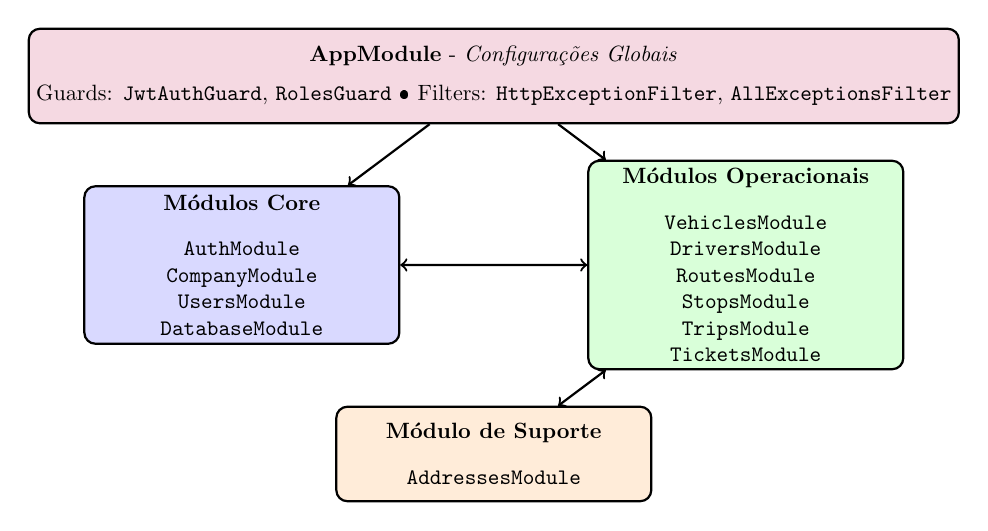
\begin{tikzpicture}[scale=0.8, every node/.style={transform shape}]
  % Módulos Core
  \node[draw, rounded corners, thick, fill=blue!15, minimum width=5cm, minimum height=2.5cm, align=center] (core) at (0,3) {
    \textbf{Módulos Core}\\[0.3cm]
    \texttt{AuthModule}\\
    \texttt{CompanyModule}\\
    \texttt{UsersModule}\\
    \texttt{DatabaseModule}
  };
  
  % Módulos Operacionais
  \node[draw, rounded corners, thick, fill=green!15, minimum width=5cm, minimum height=3cm, align=center] (operational) at (8,3) {
    \textbf{Módulos Operacionais}\\[0.3cm]
    \texttt{VehiclesModule}\\
    \texttt{DriversModule}\\
    \texttt{RoutesModule}\\
    \texttt{StopsModule}\\
    \texttt{TripsModule}\\
    \texttt{TicketsModule}
  };
  
  % Módulos de Suporte
  \node[draw, rounded corners, thick, fill=orange!15, minimum width=5cm, minimum height=1.5cm, align=center] (support) at (4,0) {
    \textbf{Módulo de Suporte}\\[0.3cm]
    \texttt{AddressesModule}
  };
  
  % AppModule
  \node[draw, rounded corners, thick, fill=purple!15, minimum width=10cm, minimum height=1.5cm, align=center] (app) at (4,6) {
    \textbf{AppModule} - \textit{Configurações Globais}\\[0.2cm]
    Guards: \texttt{JwtAuthGuard}, \texttt{RolesGuard} • Filters: \texttt{HttpExceptionFilter}, \texttt{AllExceptionsFilter}
  };
  
  % Setas
  \draw[->, thick] (app) -- (core);
  \draw[->, thick] (app) -- (operational);
  \draw[<->, thick] (core) -- (operational);
  \draw[<->, thick] (support) -- (operational);
\end{tikzpicture}
\caption{Organização modular do backend BusLy.}
\label{fig:backend-modules}
\end{figure}

\subsection{Pipeline de Processamento}

Cada requisição HTTP passa por um pipeline estruturado de middleware, guards, interceptors e filters, garantindo segurança e consistência.

\begin{figure}[H]
\centering
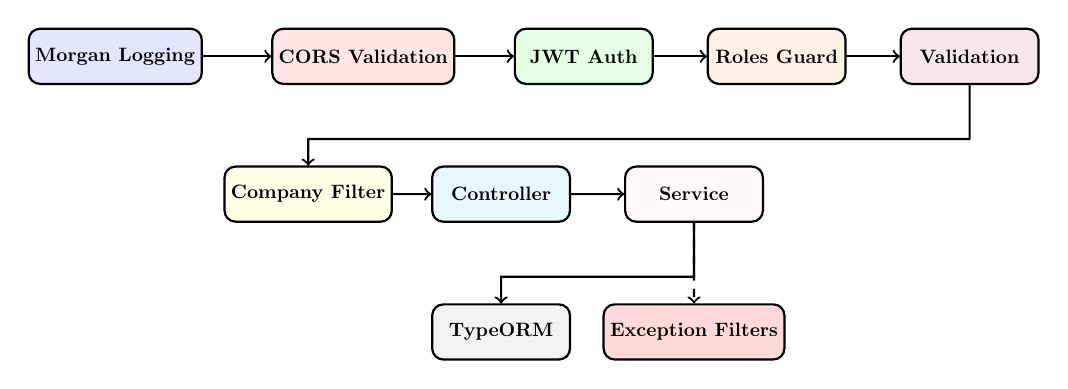
\begin{tikzpicture}[scale=0.7, every node/.style={transform shape}]
  % Pipeline stages
  \node[draw, rounded corners, thick, fill=blue!10, minimum width=2.5cm, minimum height=1cm] (morgan) at (0,0) {\textbf{Morgan Logging}};
  \node[draw, rounded corners, thick, fill=red!10, minimum width=2.5cm, minimum height=1cm] (cors) at (4.5,0) {\textbf{CORS Validation}};
  \node[draw, rounded corners, thick, fill=green!10, minimum width=2.5cm, minimum height=1cm] (jwt) at (8.5,0) {\textbf{JWT Auth}};
  \node[draw, rounded corners, thick, fill=orange!10, minimum width=2.5cm, minimum height=1cm] (roles) at (12,0) {\textbf{Roles Guard}};
  \node[draw, rounded corners, thick, fill=purple!10, minimum width=2.5cm, minimum height=1cm] (validation) at (15.5,0) {\textbf{Validation}};
  
  \node[draw, rounded corners, thick, fill=yellow!10, minimum width=3cm, minimum height=1cm] (interceptor) at (3.5,-2.5) {\textbf{Company Filter}};
  \node[draw, rounded corners, thick, fill=cyan!10, minimum width=2.5cm, minimum height=1cm] (controller) at (7,-2.5) {\textbf{Controller}};
  \node[draw, rounded corners, thick, fill=pink!10, minimum width=2.5cm, minimum height=1cm] (service) at (10.5,-2.5) {\textbf{Service}};
  
  \node[draw, rounded corners, thick, fill=gray!10, minimum width=2.5cm, minimum height=1cm] (typeorm) at (7,-5) {\textbf{TypeORM}};
  \node[draw, rounded corners, thick, fill=red!15, minimum width=3cm, minimum height=1cm] (filters) at (10.5,-5) {\textbf{Exception Filters}};
  
  % Arrows
  \draw[->, thick] (morgan) -- (cors);
  \draw[->, thick] (cors) -- (jwt);
  \draw[->, thick] (jwt) -- (roles);
  \draw[->, thick] (roles) -- (validation);
  \draw[->, thick] (validation) -- ++(0,-1.5) -| (interceptor);
  \draw[->, thick] (interceptor) -- (controller);
  \draw[->, thick] (controller) -- (service);
  \draw[->, thick] (service) -- ++(0,-1.5) -| (typeorm);
  \draw[->, thick, dashed] (service) -- (filters);
\end{tikzpicture}
\caption{Pipeline de processamento de requisições.}
\label{fig:request-pipeline}
\end{figure}

\subsection{Fluxo de Autenticação}

O sistema utiliza autenticação baseada em JWT com suporte a multi-tenancy. A Figura~\ref{fig:auth-sequence} detalha o processo completo.

\begin{figure}[H]
\centering
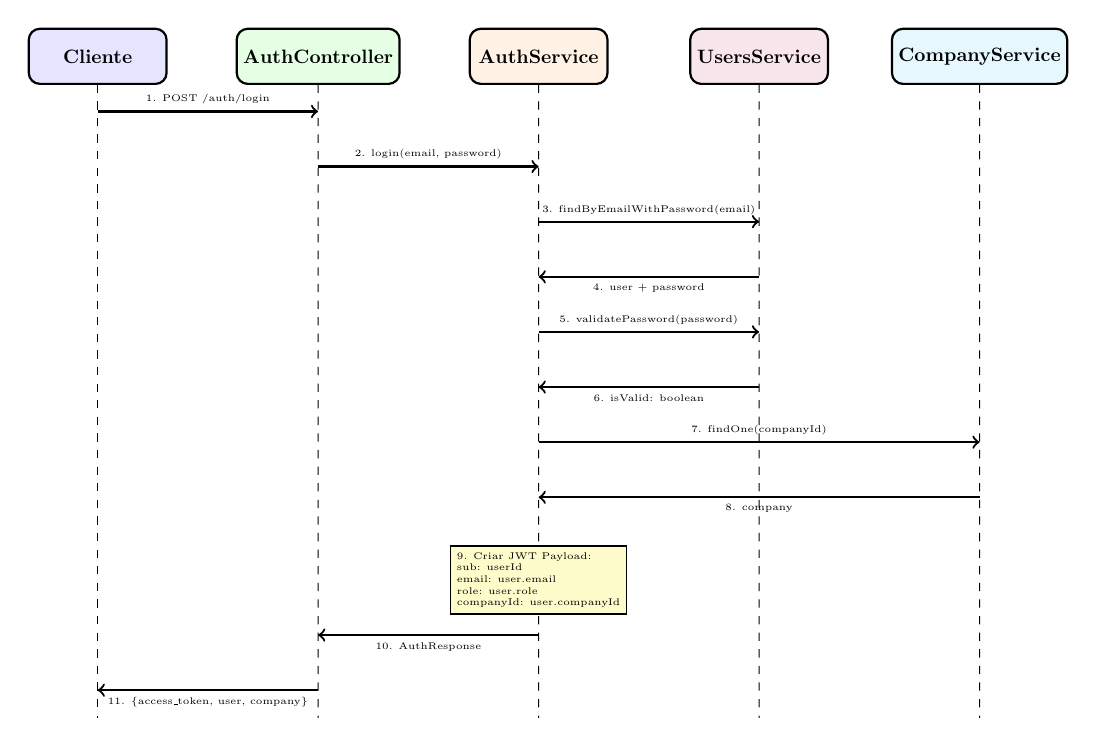
\begin{tikzpicture}[scale=0.7, every node/.style={transform shape}]
  % Participantes
  \node[draw, rounded corners, thick, fill=blue!10, minimum width=2.5cm, minimum height=1cm] (client) at (0,11) {\textbf{Cliente}};
  \node[draw, rounded corners, thick, fill=green!10, minimum width=2.5cm, minimum height=1cm] (auth) at (4,11) {\textbf{AuthController}};
  \node[draw, rounded corners, thick, fill=orange!10, minimum width=2.5cm, minimum height=1cm] (service) at (8,11) {\textbf{AuthService}};
  \node[draw, rounded corners, thick, fill=purple!10, minimum width=2.5cm, minimum height=1cm] (users) at (12,11) {\textbf{UsersService}};
  \node[draw, rounded corners, thick, fill=cyan!10, minimum width=2.5cm, minimum height=1cm] (company) at (16,11) {\textbf{CompanyService}};
  
  % Linhas de vida
  \draw[dashed] (client) -- (0,-1);
  \draw[dashed] (auth) -- (4,-1);
  \draw[dashed] (service) -- (8,-1);
  \draw[dashed] (users) -- (12,-1);
  \draw[dashed] (company) -- (16,-1);
  
  % Mensagens
  \draw[->, thick] (0,10) -- node[above, font=\tiny]{1. POST /auth/login} (4,10);
  \draw[->, thick] (4,9) -- node[above, font=\tiny]{2. login(email, password)} (8,9);
  \draw[->, thick] (8,8) -- node[above, font=\tiny]{3. findByEmailWithPassword(email)} (12,8);
  \draw[<-, thick] (8,7) -- node[below, font=\tiny]{4. user + password} (12,7);
  \draw[->, thick] (8,6) -- node[above, font=\tiny]{5. validatePassword(password)} (12,6);
  \draw[<-, thick] (8,5) -- node[below, font=\tiny]{6. isValid: boolean} (12,5);
  \draw[->, thick] (8,4) -- node[above, font=\tiny]{7. findOne(companyId)} (16,4);
  \draw[<-, thick] (8,3) -- node[below, font=\tiny]{8. company} (16,3);
  
  % Processamento interno
  \node[draw, fill=yellow!20, align=left, font=\tiny] at (8,1.5) {9. Criar JWT Payload:\\sub: userId\\email: user.email\\role: user.role\\companyId: user.companyId};
  
  \draw[<-, thick] (4,0.5) -- node[below, font=\tiny]{10. AuthResponse} (8,0.5);
  \draw[<-, thick] (0,-0.5) -- node[below, font=\tiny]{11. \{access\_token, user, company\}} (4,-0.5);
\end{tikzpicture}
\caption{Diagrama de sequência - fluxo de autenticação.}
\label{fig:auth-sequence}
\end{figure}

\subsection{Arquitetura Multi-tenant}

O sistema implementa isolamento de dados por empresa através do padrão \texttt{BaseCompanyService}, que injeta automaticamente o \texttt{companyId} em todas as operações de banco de dados. O \texttt{CompanyFilterInterceptor} extrai o contexto da empresa do token JWT e disponibiliza para os serviços.

\begin{itemize}
  \item \textbf{Isolamento Automático}: Todas as entidades operacionais possuem \texttt{companyId}
  \item \textbf{Herança de Comportamento}: Services estendem \texttt{BaseCompanyService<T>}
  \item \textbf{Contexto de Requisição}: Interceptor injeta \texttt{companyId} baseado no token JWT
  \item \textbf{Validação de Acesso}: Queries automáticas com filtro por empresa
\end{itemize}

\section{Arquitetura do Frontend}
O frontend emprega Next.js~15 (React~19) com App Router, compondo páginas e layouts por segmentos de negócio (\texttt{/dashboard/[company]/...}). Destacam-se:

\begin{itemize}
  \item \textbf{Sessão e Contexto}: NextAuth com \textit{credentials provider}; o token JWT é persistido na sessão e exposto a componentes via \texttt{useSession} e por um contexto de autenticação.
  \item \textbf{Serviços de API}: um cliente consolidado (\texttt{api.service.ts}) monta a URL base (\texttt{NEXT\_PUBLIC\_API\_URL}), anexa o token \texttt{Bearer}, trata erros e respostas padronizadas e redireciona para login em caso de 401.
  \item \textbf{Camada de UI}: biblioteca de componentes com Radix UI e Tailwind CSS, compondo tabelas, diálogos e formulários tipados com React Hook Form e Zod.
  \item \textbf{Mapas e Geografia}: Leaflet/React-Leaflet para visualização e edição de rotas e paradas (componentes de mapa, formulários e tabelas integrados).
  \item \textbf{Organização por Domínio}: páginas e componentes agrupados por recursos (empresas, motoristas, veículos, rotas, viagens, bilhetes) favorecem coesão e evolução incremental.
\end{itemize}

Essa arquitetura promove: (i) separação de preocupações, (ii) segurança com \textit{JWT} e papéis, (iii) multiempresa por chave de escopo e (iv) escalabilidade via modularização e tipagem estática de ponta a ponta.

\chapter{Apresentação do Protótipo Funcional}
\label{cha:funcionalidades}

Este capítulo apresenta a materialização do sistema ViaBus através de seu protótipo funcional de \textit{frontend}. O objetivo aqui não é apenas exibir as telas desenvolvidas, mas demonstrar como as funcionalidades implementadas atendem diretamente aos Requisitos Funcionais (RF) definidos no Capítulo~\ref{cha:requisitos}, solucionando os problemas operacionais identificados na pesquisa de mercado.

A interface foi desenvolvida seguindo os princípios de usabilidade e \textit{design} responsivo (RNF01, RNF02), garantindo uma experiência de usuário clara e consistente em diferentes dispositivos. As seções a seguir estão organizadas de acordo com o fluxo de trabalho de um gestor: o \textit{onboarding} inicial, o gerenciamento dos recursos da empresa e, por fim, a execução das operações diárias.

\section{Onboarding e Visão Geral do Sistema}

A primeira interação do usuário com o sistema envolve a autenticação e o acesso ao painel de controle, que fornece uma visão geral das operações.

\subsubsection{Autenticação e Criação de Empresa}
Para garantir a segurança e o isolamento dos dados (RNF05, RNF06), o sistema implementa um fluxo de autenticação via e-mail e senha, gerenciado pelo NextAuth, conforme visto na Figura~\ref{fig:tela-login}. No primeiro acesso, o usuário é guiado por um formulário para cadastrar os dados de sua empresa (Figura~\ref{fig:criacao-empresa}), estabelecendo o ambiente de trabalho multi-tenant.

\begin{figure}[H]
  \centering
  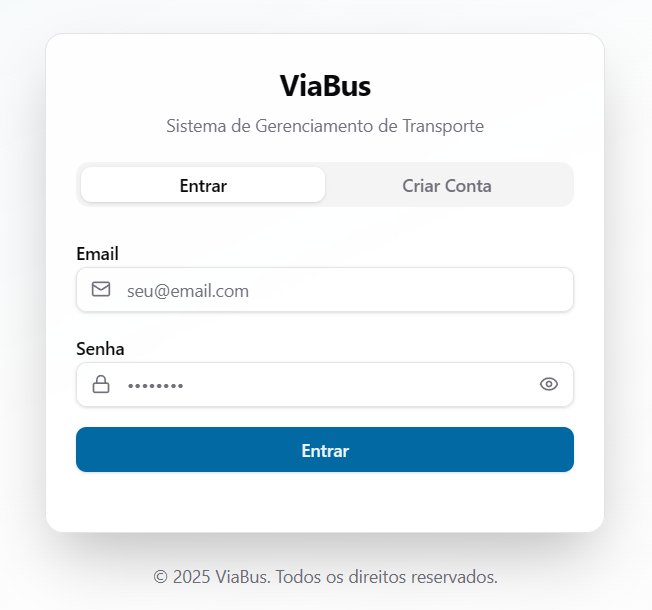
\includegraphics[width=0.6\textwidth]{imagens/tela-login.png}
  \caption{Tela de login do sistema ViaBus.}
  \label{fig:tela-login}
\end{figure}

\begin{figure}[H]
  \centering
  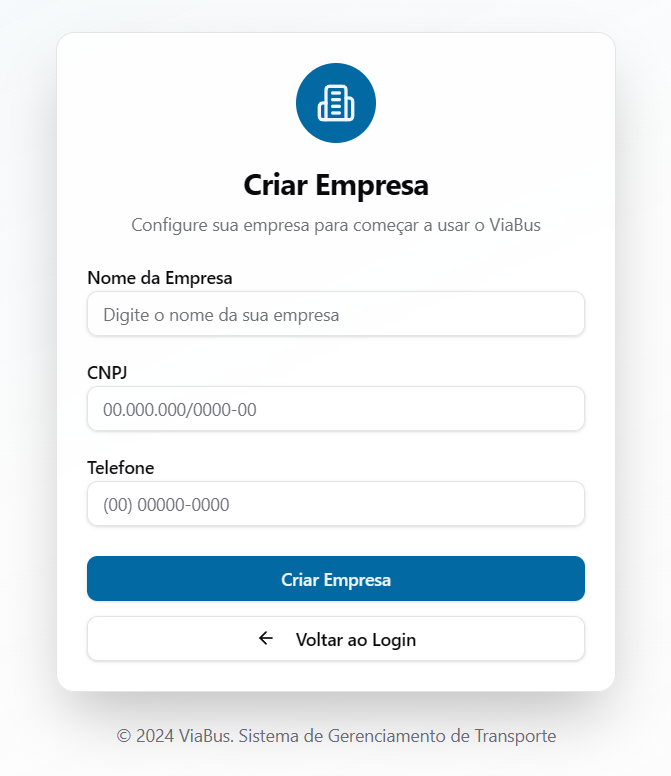
\includegraphics[width=0.6\textwidth]{imagens/criacao-empresa.png}
  \caption{Formulário de criação de empresa.}
  \label{fig:criacao-empresa}
\end{figure}

\subsubsection{Painel de Controle (Dashboard)}
Após o login, o gestor acessa o painel de controle (\textit{dashboard}), que foi concebido para atender ao requisito de \textbf{RF10} (visualizar rapidamente a ocupação e outras métricas). A interface, apresentada na Figura~\ref{fig:dashboard}, serve como uma central de comando visual para o gestor.

Nesta fase do protótipo, o \textit{layout} apresenta uma representação visual dos principais indicadores da operação. O \textit{design} foi projetado para, em futuras iterações, exibir cartões com dados consolidados e atualizados em tempo real, como o número de viagens, passagens vendidas, e o status de veículos e motoristas. O objetivo destes componentes é oferecer ao gestor um panorama instantâneo para a tomada de decisões estratégicas.

\begin{figure}[H]
  \centering
  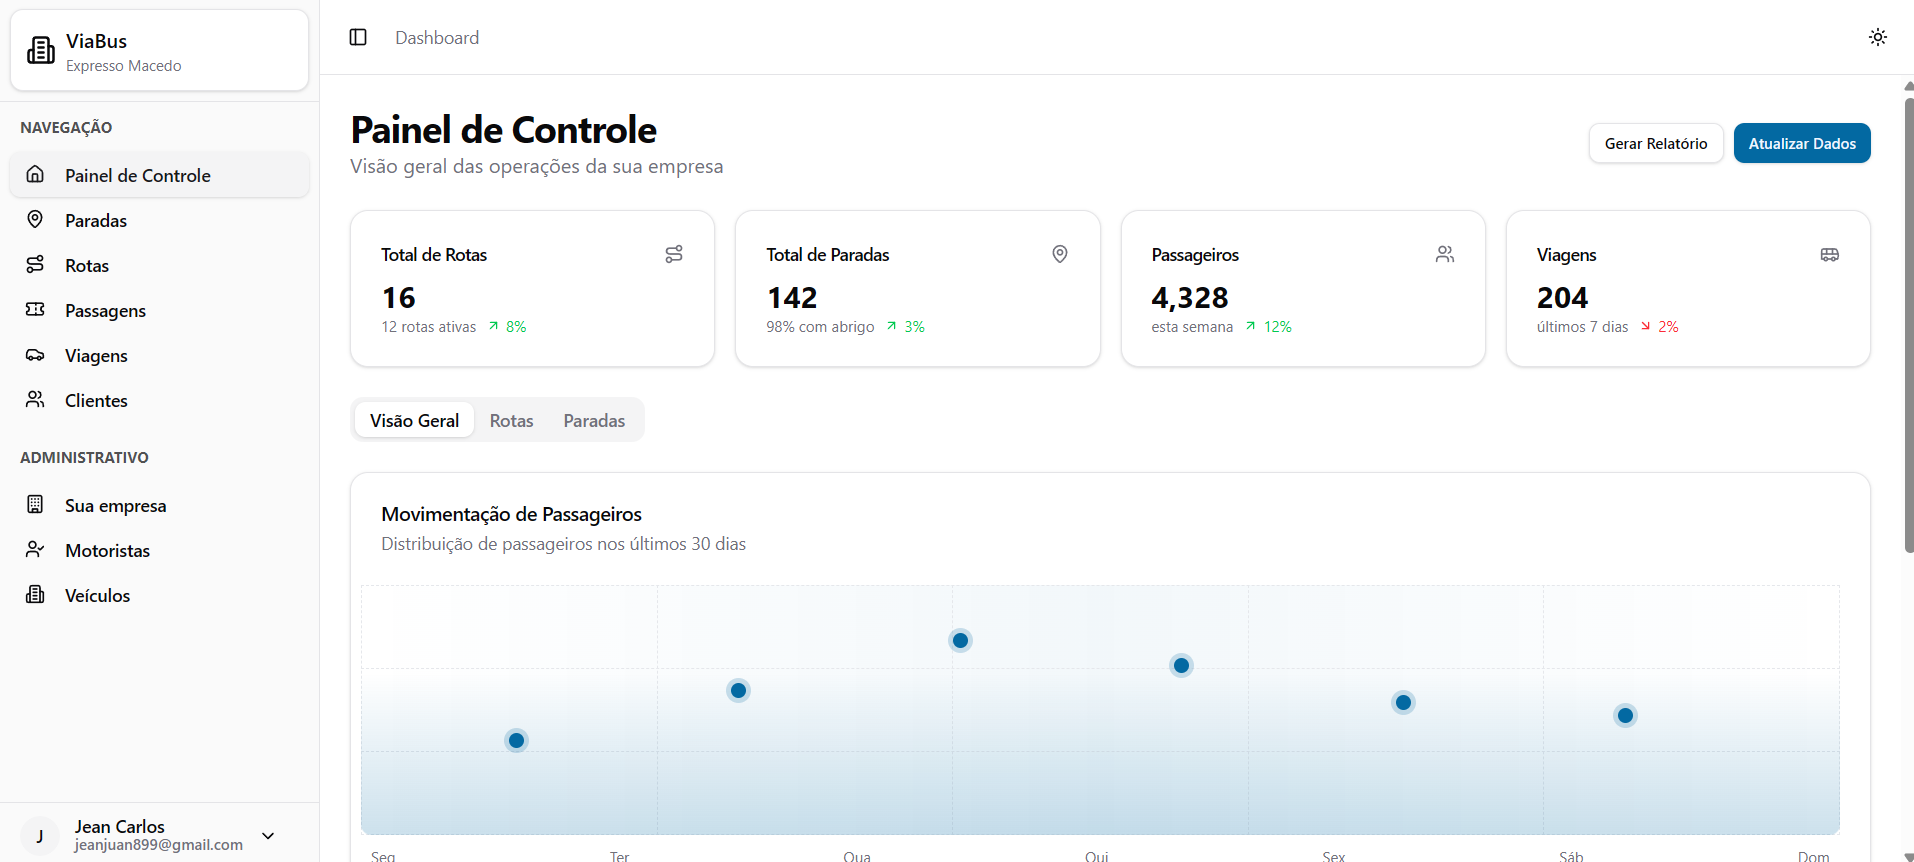
\includegraphics[width=1\textwidth]{imagens/dashboard.png}
  \caption{Painel de controle principal com métricas e navegação.}
  \label{fig:dashboard}
\end{figure}

\section{Gerenciamento de Recursos Operacionais}

Uma vez dentro do sistema, o gestor precisa configurar os recursos fundamentais de sua operação. Esta seção demonstra as interfaces criadas para o cadastro de paradas, rotas, veículos e motoristas.

\subsubsection{Gestão de Paradas e Rotas}
Para atender aos requisitos \textbf{RF03} (cadastro de pontos de parada) e \textbf{RF04} (organização de rotas), foram desenvolvidos módulos específicos. A Figura~\ref{fig:listagem-paradas} exibe a tela de listagem de paradas, enquanto a Figura~\ref{fig:formulario-parada} demonstra o formulário de cadastro, que integra um mapa interativo para facilitar a definição precisa da localização. Em seguida, na interface de criação de rotas (Figura~\ref{fig:criacao-rota}), o gestor pode selecionar essas paradas em uma sequência lógica para formar um itinerário.

\begin{figure}[H]
  \centering
  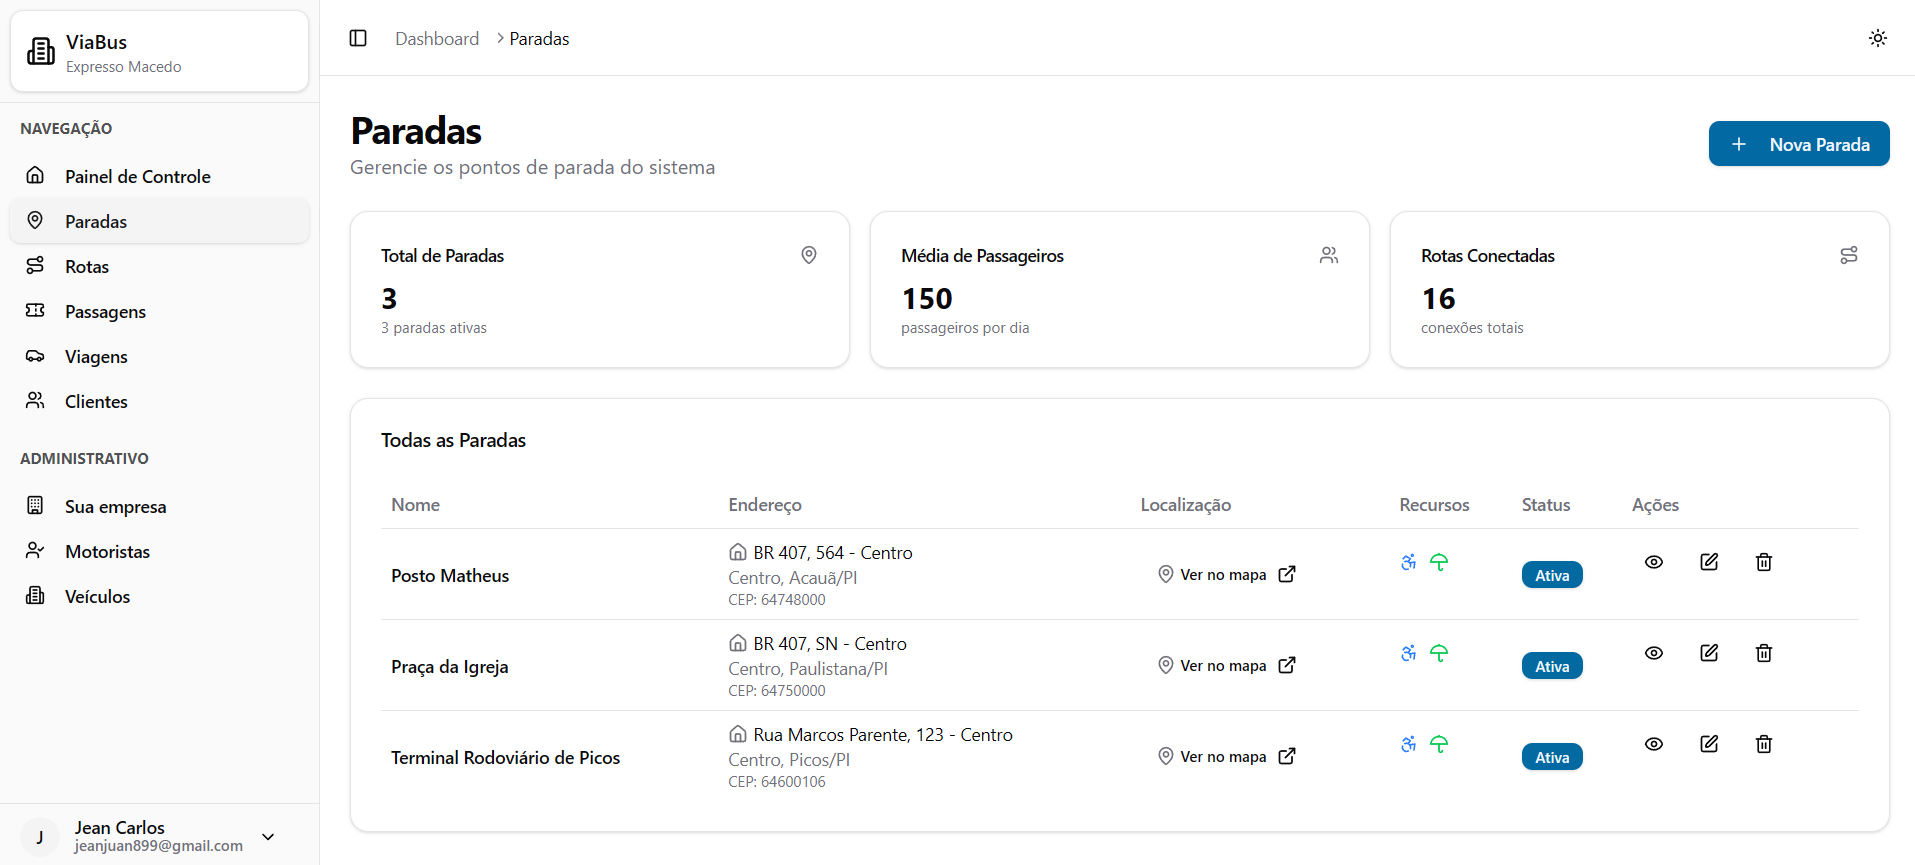
\includegraphics[width=1\textwidth]{imagens/listagem-paradas.png}
  \caption{Listagem de paradas com funcionalidades de busca e filtros.}
  \label{fig:listagem-paradas}
\end{figure}

\begin{figure}[H]
  \centering
  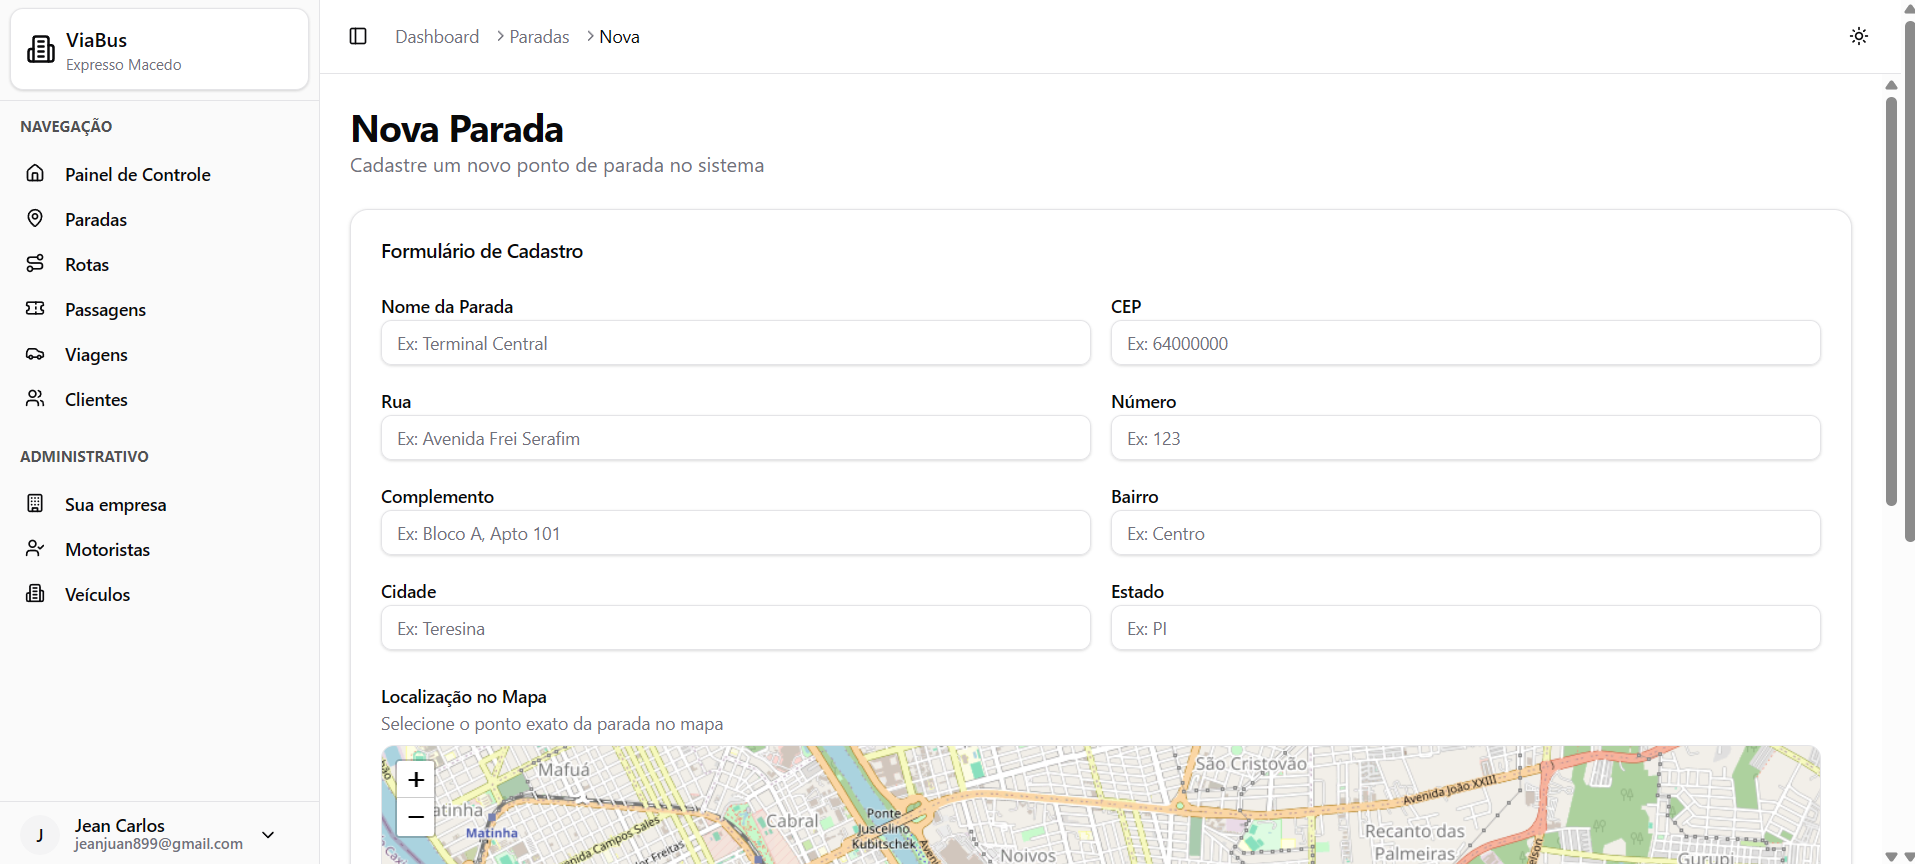
\includegraphics[width=1\textwidth]{imagens/formulario-parada.png}
  \caption{Formulário de cadastro de parada com mapa interativo.}
  \label{fig:formulario-parada}
\end{figure}

\begin{figure}[H]
  \centering
  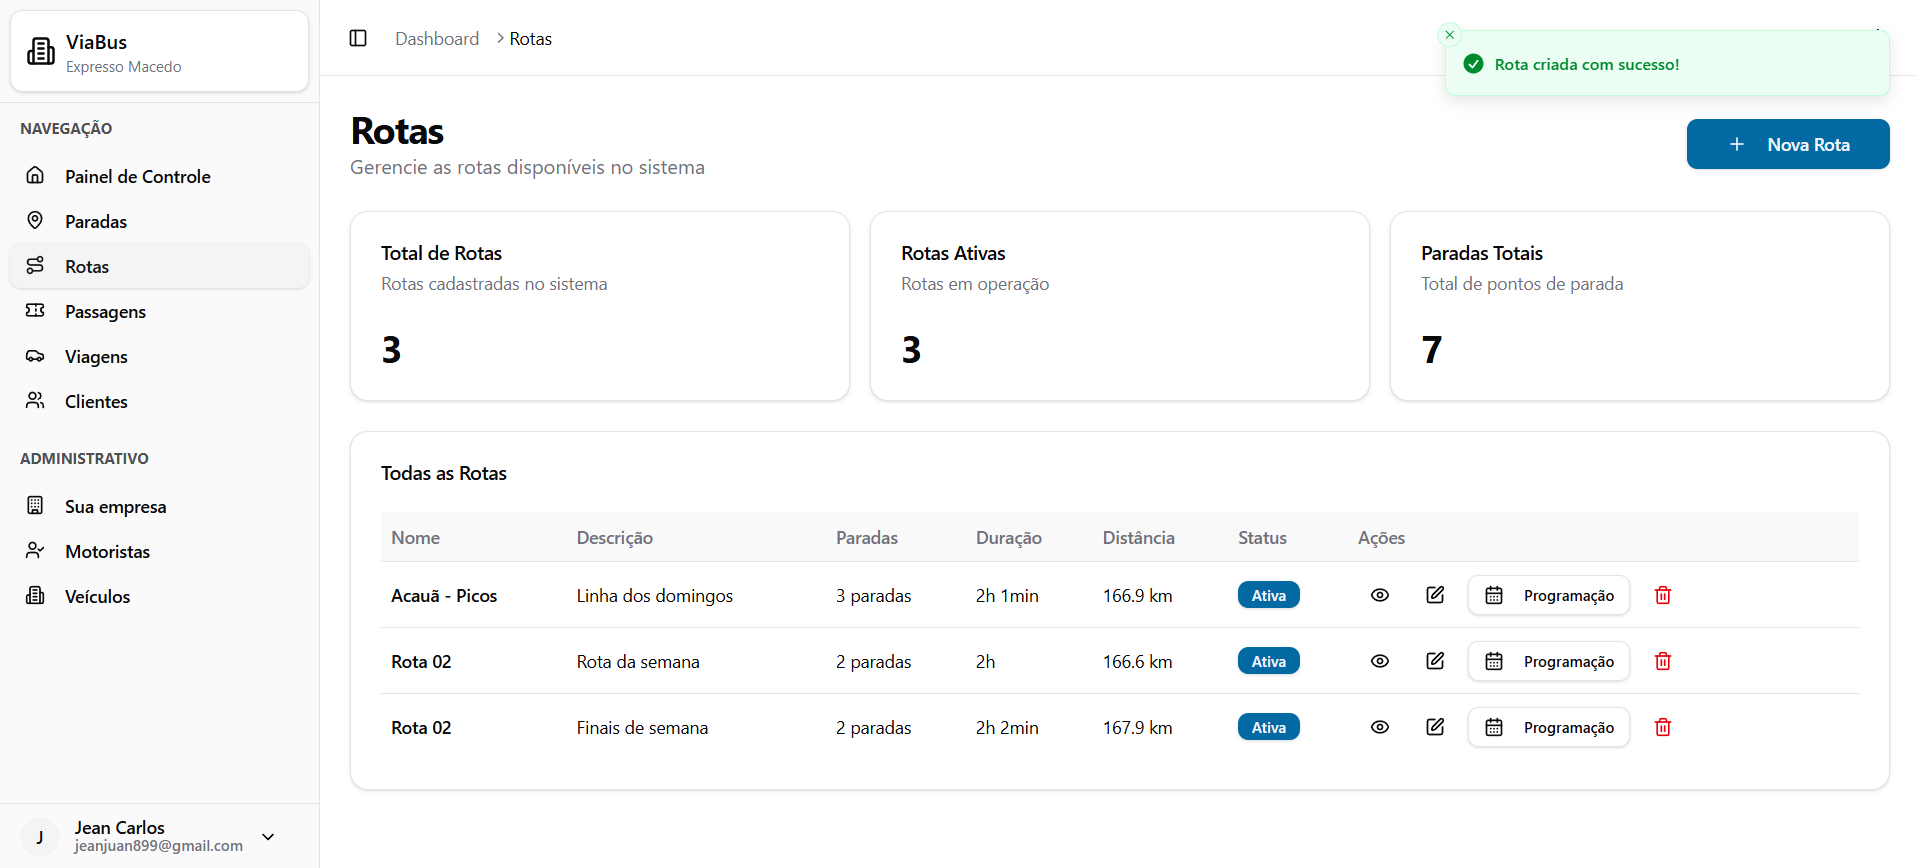
\includegraphics[width=1\textwidth]{imagens/tela-rotas.png}
  \caption{Listagem de rotas com funcionalidades de busca e filtros.}
  \label{fig:tela-rotas}
\end{figure}

\begin{figure}[H]
  \centering
  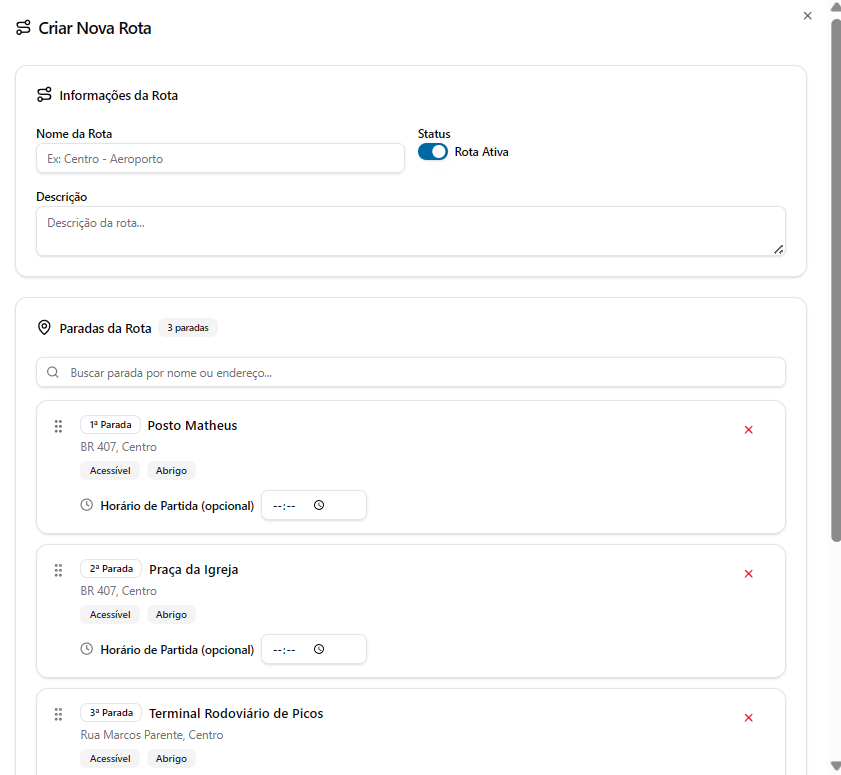
\includegraphics[width=0.7\textwidth]{imagens/criacao-rota.png}
  \caption{Interface de criação de rota com seleção de paradas.}
  \label{fig:criacao-rota}
\end{figure}

\subsubsection{Gestão da Frota e de Motoristas}
Atendendo aos requisitos \textbf{RF01} (gerenciar frota) e \textbf{RF02} (gerenciar motoristas), o sistema oferece interfaces dedicadas para o controle de veículos e condutores. As Figuras~\ref{fig:veiculos} e \ref{fig:motoristas} mostram as telas de listagem, onde é possível consultar informações detalhadas, verificar o status operacional de cada recurso e realizar ações de gerenciamento.

\begin{figure}[H]
  \centering
  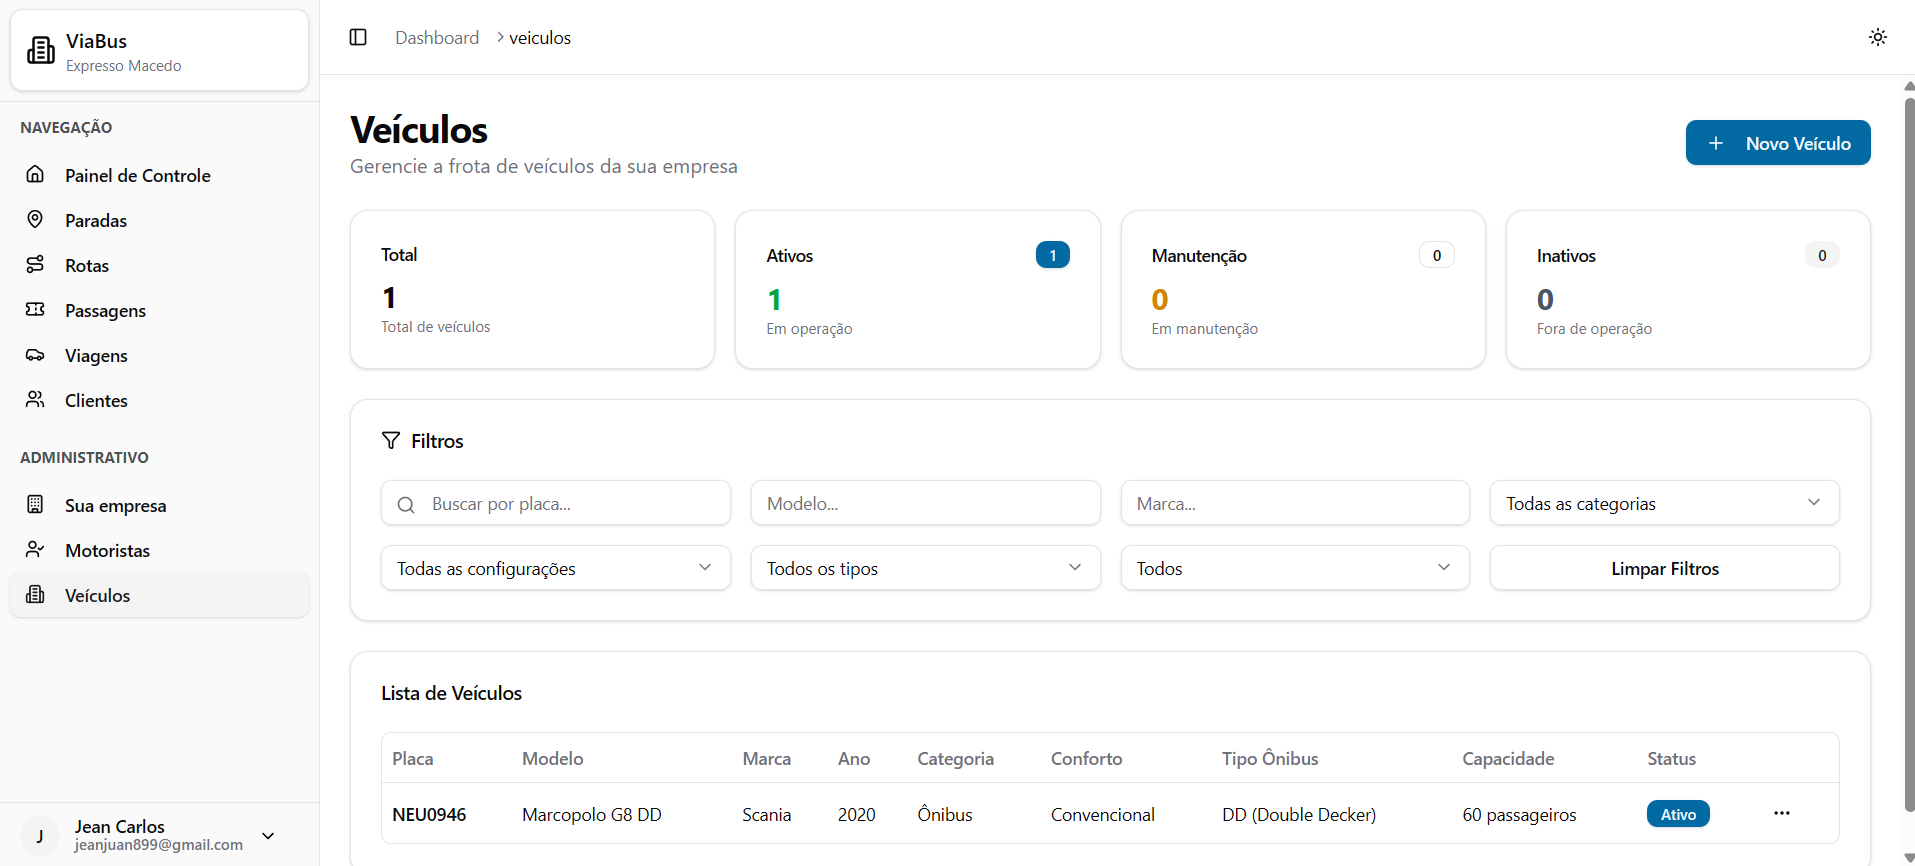
\includegraphics[width=1\textwidth]{imagens/veiculos.png}
  \caption{Listagem de veículos com status operacional.}
  \label{fig:veiculos}
\end{figure}

\begin{figure}[H]
  \centering
  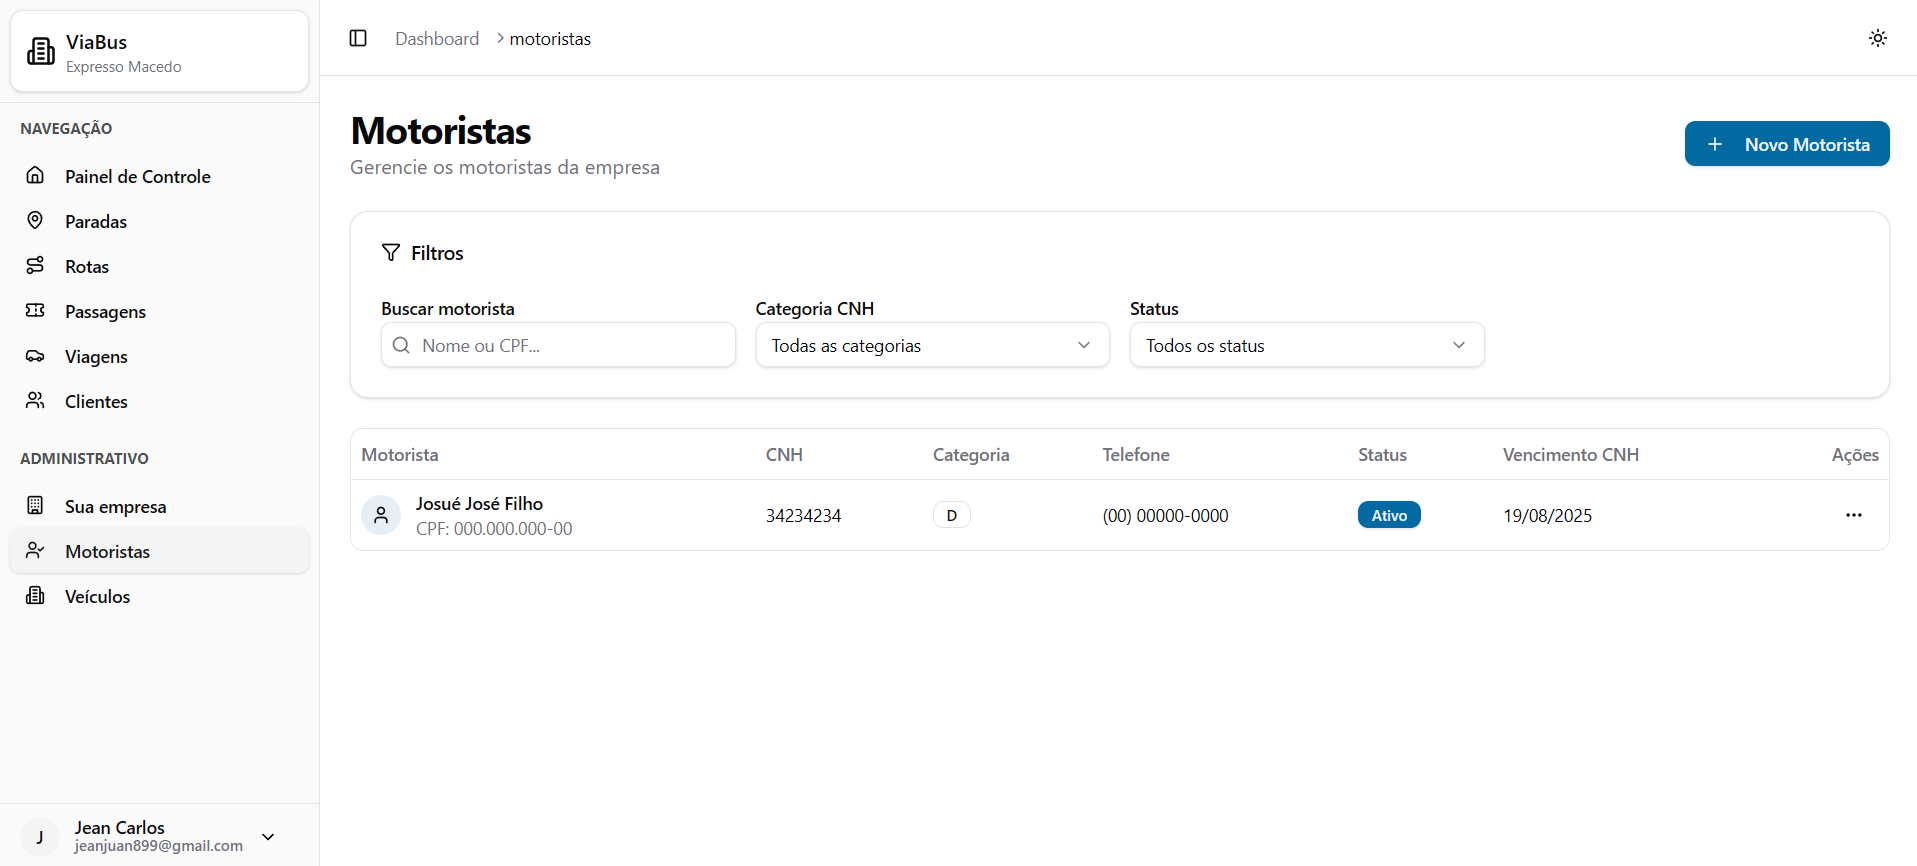
\includegraphics[width=1\textwidth]{imagens/motoristas.png}
  \caption{Interface de gerenciamento de motoristas.}
  \label{fig:motoristas}
\end{figure}

\section{Execução das Operações Diárias}

Com os recursos configurados, esta seção demonstra as funcionalidades centrais para a operação do dia a dia: o agendamento de viagens e a venda de passagens, que digitalizam o processo antes realizado em cadernos e aplicativos de mensagem.

\subsubsection{Agendamento de Viagens}
O requisito \textbf{RF05} (agendamento de viagens futuras) é materializado na interface da Figura~\ref{fig:agendamento-viagem}. Nela, o gestor pode criar uma nova viagem selecionando uma rota pré-definida e associando os recursos necessários, como o veículo e o motorista que realizarão o trajeto.

\begin{figure}[H]
  \centering
  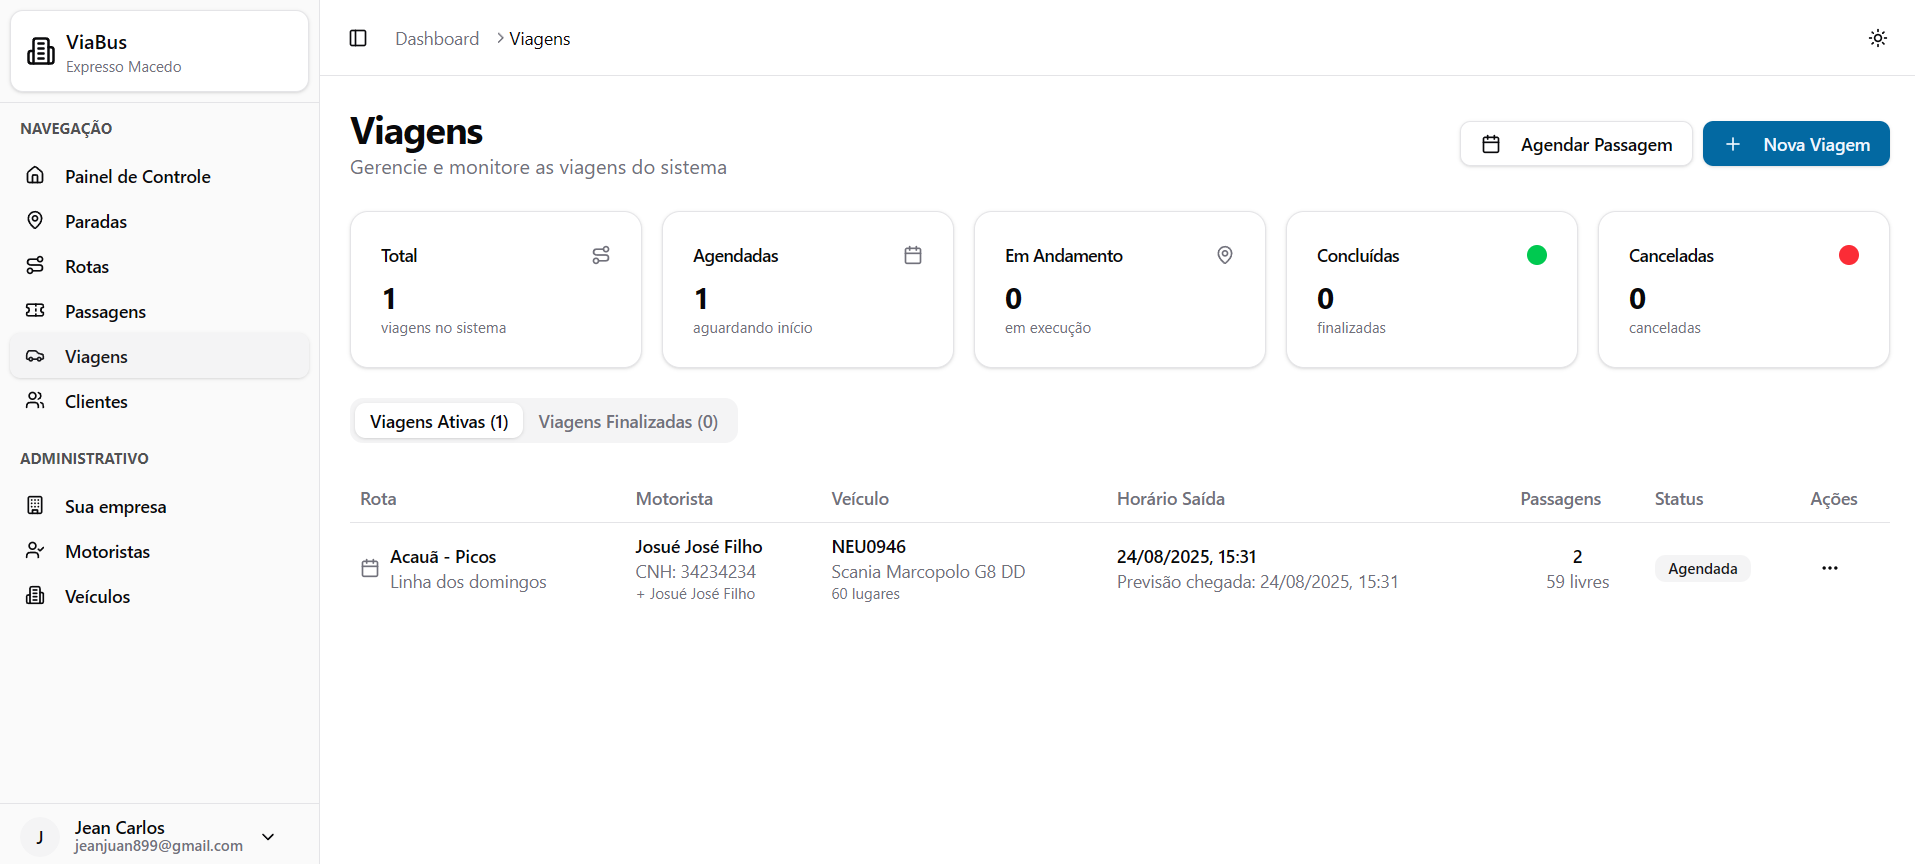
\includegraphics[width=1\textwidth]{imagens/agendamento-viagem.png}
  \caption{Processo de agendamento de viagem.}
  \label{fig:agendamento-viagem}
\end{figure}

\subsubsection{Assistente de Venda de Passagens}
O processo de venda de passagens foi projetado para ser rápido e à prova de erros, atendendo a um conjunto de requisitos essenciais. Para cumprir o \textbf{RF06} (venda rápida e guiada), foi implementado um assistente (\textit{wizard}) em cinco etapas. O fluxo se inicia com a seleção da rota e horário (Figuras~\ref{fig:wizard-rota} e \ref{fig:wizard-data}). Em seguida, são coletadas as informações do passageiro, conforme o \textbf{RF07} (Figura~\ref{fig:wizard-passageiro}), e selecionados os locais de embarque e desembarque (Figura~\ref{fig:wizard-locais}). Durante todo o processo, o sistema valida a disponibilidade de assentos em tempo real, satisfazendo o requisito crítico \textbf{RF08} (evitar overbooking). A etapa final (Figura~\ref{fig:wizard-confirmacao}) resume a venda e gera o bilhete, que pode ser usado para compor a lista de passageiros do \textbf{RF09}.

\begin{figure}[H]
  \centering
  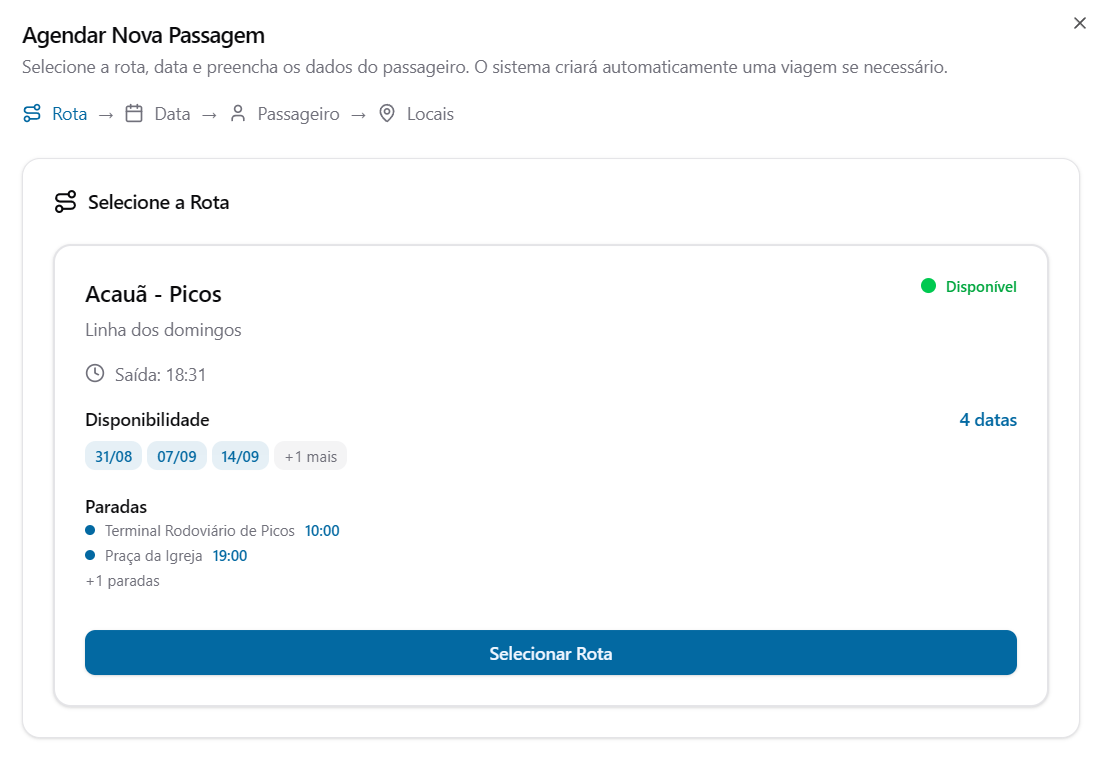
\includegraphics[width=0.8\textwidth]{imagens/wizard-rota.png}
  \caption{Seleção de rota no wizard de passagens.}
  \label{fig:wizard-rota}
\end{figure}

\begin{figure}[H]
  \centering
  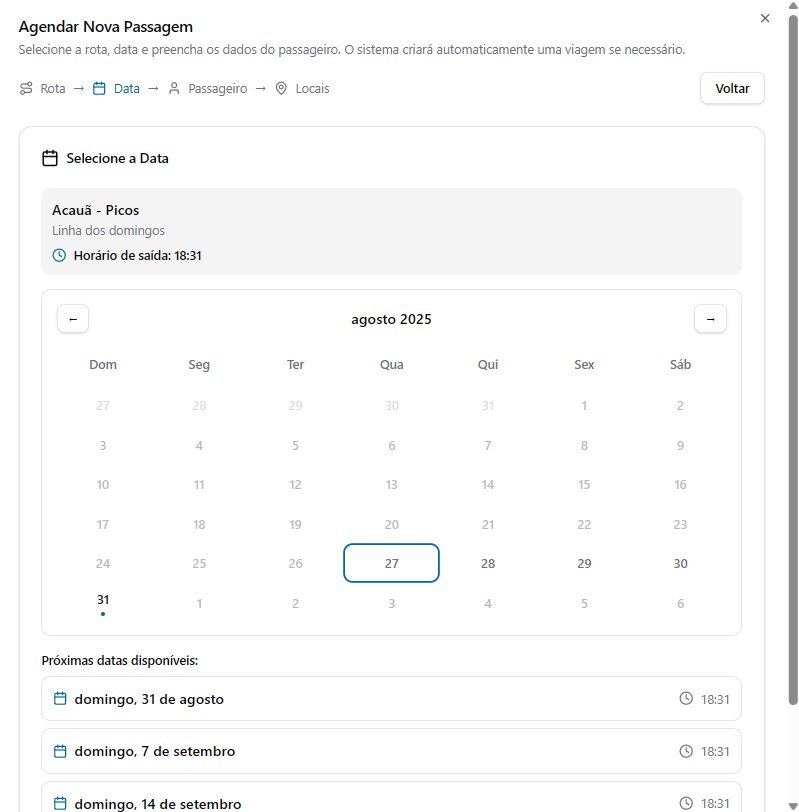
\includegraphics[width=0.6\textwidth]{imagens/wizard-data.png}
  \caption{Seleção de data e horário.}
  \label{fig:wizard-data}
\end{figure}

\begin{figure}[H]
  \centering
  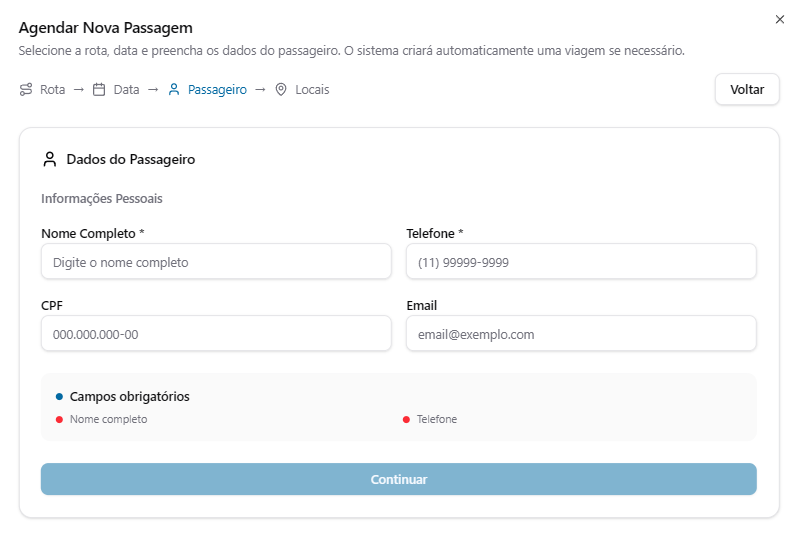
\includegraphics[width=0.8\textwidth]{imagens/wizard-passageiro.png}
  \caption{Cadastro de informações do passageiro.}
  \label{fig:wizard-passageiro}
\end{figure}

\begin{figure}[H]
  \centering
  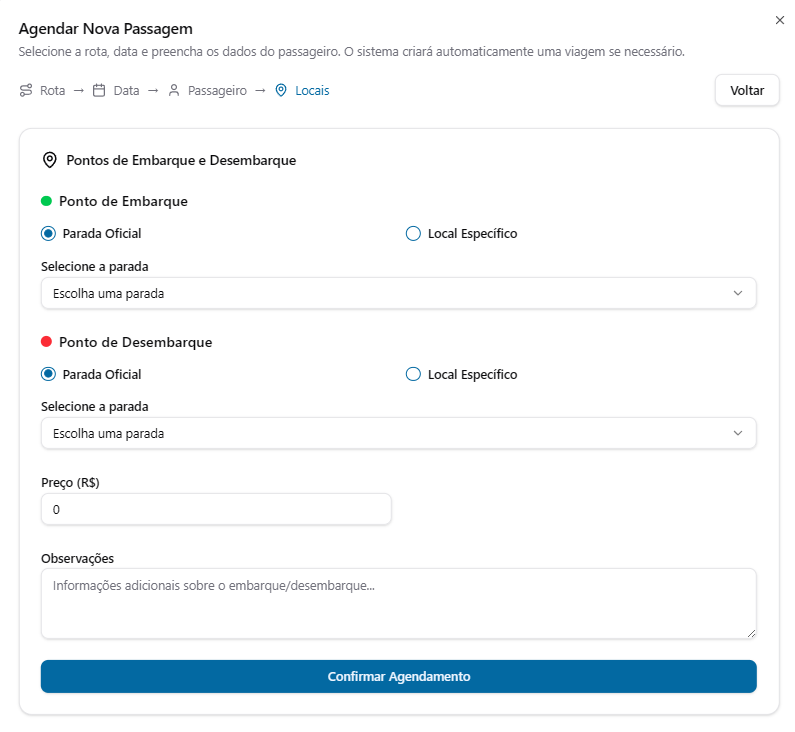
\includegraphics[width=0.7\textwidth]{imagens/wizard-locais.png}
  \caption{Seleção de locais de embarque e desembarque.}
  \label{fig:wizard-locais}
\end{figure}

\begin{figure}[H]
  \centering
  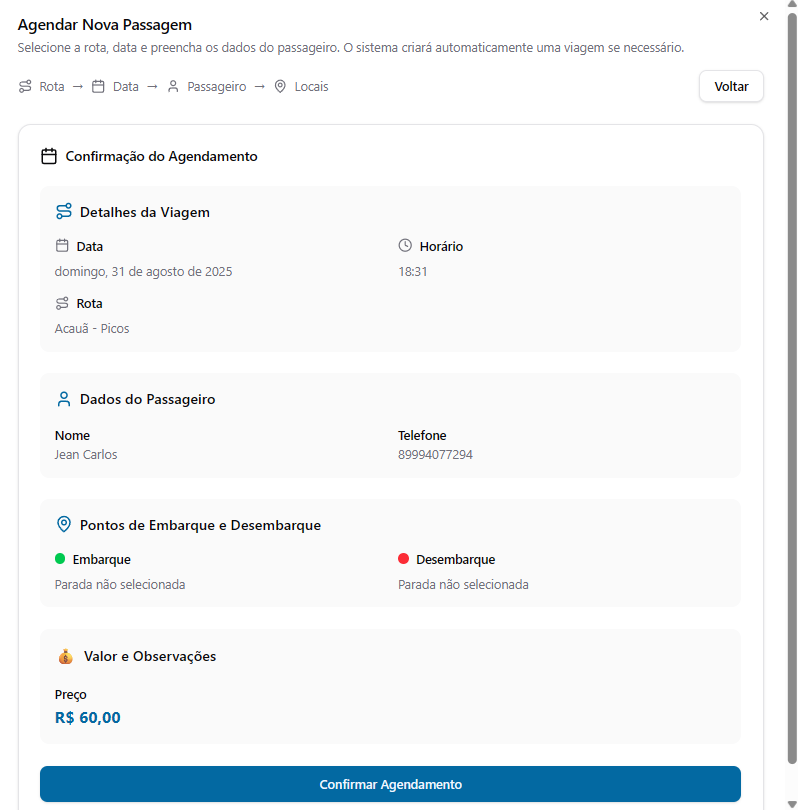
\includegraphics[width=0.7\textwidth]{imagens/wizard-confirmacao.png}
  \caption{Confirmação final e geração da passagem.}
  \label{fig:wizard-confirmacao}
\end{figure}


\chapter{Resultados e Discussão}\label{cha:resultados}

\section{Verificação de Requisitos}

A primeira etapa da avaliação consistiu na verificação sistemática do grau de implementação dos Requisitos Funcionais (RF) e Não Funcionais (RNF) definidos no Capítulo 3. A análise buscou constatar se as funcionalidades e características planejadas foram efetivamente traduzidas em software. As Tabelas \ref{tab:verificacao-rf} e \ref{tab:verificacao-rnf} apresentam o resultado consolidado desta verificação.

\begin{table}[htbp]
  \centering
  \caption{Verificação dos Requisitos Funcionais (RF)}
  \label{tab:verificacao-rf}
  \resizebox{\textwidth}{!}{%
    \begin{tabular}{|l|c|p{9.5cm}|}
      \hline
      \textbf{Requisito}             & \textbf{Status}           & \textbf{Observações e Evidências}                                                                        \\
      \hline
      RF01 -- Registro               & Implementado              & Fluxo de cadastro de usuários disponível na API de autenticação, com validação de dados.                 \\
      RF02 -- Login                  & Implementado              & Autenticação via e-mail e senha com emissão de JWT e proteção de rotas.                                  \\
      RF03 -- Permissões             & Implementado              & Controle de acesso por perfis/roles com guards no backend e proteção de rotas no frontend.               \\
      RF04 -- Empresas               & Implementado              & Criação e gestão de perfis de empresa disponíveis; página de criação de empresa no frontend.             \\
      RF05 -- Isolamento             & Implementado              & Interceptor/serviço central aplica filtro por \textit{companyId} do usuário em todas as requisições.     \\
      RF06 -- Motoristas             & Implementado              & CRUD completo de motoristas no módulo dedicado.                                                          \\
      RF07 -- Veículos               & Implementado              & CRUD completo de veículos no módulo dedicado.                                                            \\
      RF08 -- Paradas                & Implementado              & CRUD de pontos de parada com armazenamento de geolocalização.                                            \\
      RF09 -- Rotas                  & Implementado              & Criação e manutenção de rotas com sequência de paradas.                                                  \\
      RF10 -- Horários               & Parcialmente Implementado & Associação de horários e preços às rotas; serviços de \textit{schedules} no frontend.                    \\
      RF11 -- Mapas                  & Parcialmente Implementado & Visualização de rotas e paradas disponível; ausência de mapa interativo avançado em algumas telas.       \\
      RF12 -- Agendamento de Viagens & Implementado              & Criação de viagens baseada em rotas e horários no módulo de viagens.                                     \\
      RF13 -- Atribuição             & Implementado              & Associação de veículos e motoristas às viagens.                                                          \\
      RF14 -- Status de Viagens      & Parcialmente Implementado & Atualização de status disponível; sem comunicação em tempo real por WebSocket.                           \\
      RF15 -- Wizard de Venda        & Implementado              & Fluxo guiado de venda com \textit{wizard} no frontend.                                                   \\
      RF16 -- Embarque/Desembarque   & Implementado              & Seleção flexível de pontos ao longo da rota no ato da venda.                                             \\
      RF17 -- Passageiros            & Implementado              & Coleta e armazenamento dos dados completos dos passageiros.                                              \\
      RF18 -- Anti-Overbooking       & Implementado              & Verificação de disponibilidade antes da emissão; criação de ticket bloqueada com erro 409 quando lotado. \\
      RF19 -- Listas                 & Implementado              & Geração/visualização de listas de passageiros por viagem nas telas operacionais.                         \\
      RF20 -- Busca                  & Parcialmente Implementado & Filtros múltiplos disponíveis nas listagens; oportunidades de ampliar critérios e combinações.           \\
      RF21 -- Ocupação em Tempo Real & Parcialmente Implementado & Visualização de ocupação por viagem; ausência de atualização \textit{push} em tempo real.                \\
      \hline
    \end{tabular}%
  }
\end{table}

\begin{table}[htbp]
  \centering
  \caption{Verificação dos Requisitos Não Funcionais (RNF)}
  \label{tab:verificacao-rnf}
  \resizebox{\textwidth}{!}{%
    \begin{tabular}{|l|c|p{9.5cm}|}
      \hline
      \textbf{Requisito}                  & \textbf{Status}           & \textbf{Observações e Evidências}                                                         \\
      \hline
      RNF01 -- Responsividade             & Implementado              & Interface responsiva, componentes padronizados e adaptação a diferentes tamanhos de tela. \\
      RNF02 -- Navegação                  & Parcialmente Implementado & Fluxos principais claros; avaliação heurística indica melhorias na prevenção de erros.    \\
      RNF03 -- Acessibilidade             & Parcialmente Implementado & Formulários com indicadores de progresso; faltam recursos avançados de acessibilidade.    \\
      RNF04 -- Autenticação               & Implementado              & Login seguro com JWT e controle de sessão.                                                \\
      RNF05 -- Autorização                & Implementado              & Acesso baseado em perfis com guards e verificação centralizada.                           \\
      RNF06 -- Isolamento                 & Implementado              & Separação de dados por empresa garantida via filtro automático por \textit{companyId}.    \\
      RNF07 -- Validação                  & Implementado              & Validação de entrada no backend (DTOs/validators) e no frontend.                          \\
      RNF08 -- Desempenho de Carregamento & Implementado              & Páginas com tempos de resposta adequados nos fluxos críticos.                             \\
      RNF09 -- Otimização de Consultas    & Parcialmente Implementado & Consultas indexadas nos módulos principais; há espaço para otimizações adicionais.        \\
      RNF10 -- Escalabilidade             & Parcialmente Implementado & Arquitetura modular; ausência de escalonamento horizontal automático e fila de mensagens. \\
      RNF11 -- Arquitetura                & Implementado              & Código organizado por módulos com camadas bem definidas.                                  \\
      RNF12 -- Padrões                    & Implementado              & Padrões de codificação consistentes e lint configurado.                                   \\
      RNF13 -- Documentação               & Parcialmente Implementado & Documentação básica presente; falta detalhamento abrangente de API e decisões de projeto. \\
      RNF14 -- Containerização            & Implementado              & Dockerfile no frontend e backend; orquestração via \texttt{docker-compose}.               \\
      RNF15 -- Configuração de Ambientes  & Implementado              & Suporte a múltiplos ambientes com variáveis de ambiente.                                  \\
      \hline
    \end{tabular}%
  }
\end{table}

\section{Avaliação Heurística}
A segunda etapa da avaliação do protótipo consistiu em uma Avaliação Heurística, método de inspeção de usabilidade consolidado por Nielsen (1994). Atuando como avaliador especialista, foram analisados os principais fluxos de interação do sistema, como o cadastro de rotas e a venda de passagens, com o objetivo de identificar potenciais problemas e pontos de aderência a boas práticas de design de interface. A seguir, são discutidos os achados mais relevantes, agrupados pelas heurísticas correspondentes.

Visibilidade do status do sistema (Heurística 1)
O sistema se destaca na aplicação desta heurística. Em operações que demandam tempo, como o carregamento de tabelas de dados, a interface exibe componentes de skeleton loading (Figura X, a ser inserida por você, mostrando a tabela "carregando"), comunicando claramente ao usuário que uma ação está em progresso. Adicionalmente, ações de sucesso ou falha, como salvar um novo veículo, disparam notificações do tipo toast no canto da tela, como ilustrado na Figura \ref{fig:toast-success}, fornecendo feedback imediato e não intrusivo.

Correspondência entre o sistema e o mundo real (Heurística 2)
A plataforma utiliza uma linguagem e iconografia familiar ao usuário-alvo. Termos como "Frota", "Motoristas", "Paradas" e "Rotas" são diretos e correspondem à terminologia do setor. A utilização de mapas interativos para a gestão de paradas e visualização de rotas, como visto na Figura \ref{fig:mapa-paradas}, cria uma representação visual que espelha diretamente a operação logística do mundo real, facilitando o entendimento e a manipulação dos dados.

Consistência e padronização (Heurística 4)
Este é um dos pontos mais fortes do protótipo. A utilização sistemática da biblioteca de componentes shadcn/ui garante uma alta consistência visual e de interação. Elementos como botões, formulários, tabelas e modais, como o de cadastro de nova parada (Figura \ref{fig:modal-parada}), mantêm uma identidade e um comportamento padronizados em todos os módulos. Essa consistência reduz a carga cognitiva do usuário e acelera a curva de aprendizado da ferramenta.

Prevenção de erros (Heurística 5)
Neste ponto, foram identificadas oportunidades de melhoria. No formulário de criação de rotas (Figura \ref{fig:form-rotas}), o sistema atualmente permite que o usuário avance e tente salvar uma rota sem ter selecionado nenhuma parada. Isso representa um erro potencial, pois uma rota sem paradas é funcionalmente inútil e pode gerar dados inconsistentes. Uma melhoria recomendada seria a implementação de uma validação no frontend que desabilite o botão "Salvar" ou exiba uma mensagem de alerta enquanto a lista de paradas da rota estiver vazia.

Reconhecimento em vez de memorização (Heurística 6)
A interface faz um bom trabalho ao manter as opções e informações visíveis. O menu lateral persistente (Figura \ref{fig:sidebar}) permite que o usuário navegue entre os módulos sem precisar memorizar o caminho. No entanto, no fluxo de venda de passagens, o sistema poderia melhorar ao exibir um resumo da seleção (ex: "Rota: Picos x Teresina, Data: 29/08/2025") em todos os passos do assistente, para que o usuário não precise memorizar as informações inseridas nos passos anteriores.

Estética e design minimalista (Heurística 8)
A interface do ViaBus é limpa e funcional. Não há excesso de informações ou elementos visuais que possam distrair o usuário de suas tarefas. O uso de espaços em branco e a hierarquia visual clara, como visto no Dashboard (Figura \ref{fig:dashboard}), contribuem para um design minimalista que prioriza o conteúdo e a funcionalidade.

\section{Discussão dos Resultados}

Lorem ipsum dolor sit amet, consectetur adipiscing elit. Sed do eiusmod tempor incididunt ut labore et dolore magna aliqua. Ut enim ad minim veniam, quis nostrud exercitation ullamco laboris nisi ut aliquip ex ea commodo consequat. Duis aute irure dolor in reprehenderit in voluptate velit esse cillum dolore eu fugiat nulla pariatur. Excepteur sint occaecat cupidatat non proident, sunt in culpa qui officia deserunt mollit anim id est laborum.
\chapter{Considerações Finais}
\label{cha:consideracoes_finais}

Este trabalho de conclusão de curso abordou o desafio da gestão operacional no setor de transporte rodoviário alternativo de passageiros, um segmento caracterizado pela carência de soluções tecnológicas acessíveis. O problema central identificado foi a dependência de métodos manuais e fragmentados, que resultam em ineficiências e risco de erros. Diante deste cenário, o objetivo geral do projeto foi desenvolver um protótipo funcional de uma plataforma web, no modelo \textit{Software as a Service} (SaaS), denominada ViaBus, para centralizar e digitalizar essa gestão.

\section{Conclusão}

Conclui-se que o objetivo geral do trabalho foi atingido, uma vez que o protótipo funcional foi desenvolvido e sua arquitetura, detalhada. A implementação materializou os requisitos essenciais levantados na pesquisa de mercado — como o gerenciamento de recursos e a execução de operações de venda —, demonstrando que a abordagem técnica proposta é uma solução plausível para o problema. As contribuições deste projeto são, portanto, de ordem prática e documental: o próprio protótipo funcional, que serve como prova de conceito, e a documentação de uma proposta de arquitetura para a construção de um sistema SaaS \textit{multi-tenant} focado neste nicho de mercado.

\section{Limitações do Trabalho}

É fundamental reconhecer as limitações inerentes a este trabalho para contextualizar o alcance de suas conclusões. A principal limitação metodológica reside na pesquisa de mercado, conduzida com uma amostra de apenas dois gestores, o que não permite a generalização estatística dos achados. No que tange à validação, a utilização de uma Avaliação Heurística em vez de testes com usuários finais oferece conclusões de usabilidade de caráter preliminar. Por fim, o escopo do protótipo funcional foi deliberadamente focado na perspectiva do gestor, não incluindo o desenvolvimento de uma aplicação para o passageiro e motorista, funcionalidades apontadas como relevantes na pesquisa.

\section{Trabalhos Futuros}

Com base nas limitações apontadas, delineia-se um caminho claro para a evolução do projeto. Recomenda-se, primeiramente, a validação da solução em maior escala, através de uma pesquisa de mercado quantitativa e da condução de testes de usabilidade com usuários reais. Em paralelo, o desenvolvimento do protótipo pode avançar com a implementação de funcionalidades de relatório (RF11) e do manifesto de viagem para o motorista (RF09). A criação de um único e versátil aplicativo móvel que, por meio de perfis de usuário distintos, atenderia tanto ao passageiro — com funcionalidades para a compra de bilhetes e o rastreamento de viagens — quanto ao motorista — oferecendo ferramentas para o controle digital do embarque — e a integração com sistemas de pagamento online representam os passos subsequentes para transformar o protótipo em um produto de mercado.